%! program = pdflatex

\documentclass[12pt]{article}

%%% PACKAGES
\usepackage{ifpdf}
\usepackage{booktabs}   % for much better looking tables
\usepackage{array}      % for better arrays (eg matrices) in maths
\usepackage{paralist}   % very flexible & customisable lists (eg. enumerate/itemize, etc.)
%\usepackage{verbatim}   % adds environment for commenting out blocks of text & for better verbatim
\usepackage{subfigure}  % make it possible to include more than one captioned figure/table in a single float
% These packages are all incorporated in the memoir class to one degree or another...
\ifpdf
\usepackage[pdftex]{graphicx}
\else
\usepackage[dvips]{graphicx}
\fi
\usepackage{epstopdf}
\usepackage[cmex10]{amsmath}
\interdisplaylinepenalty=2500

%%% PAGE DIMENSIONS
\usepackage{geometry} % to change the page dimensions
\geometry{letterpaper}
%\geometry{margins=2in} % for example, change the margins to 2 inches all round
%\geometry{landscape} % set up the page for landscape
% read geometry.pdf for detailed page layout information

%% HEADERS & FOOTERS
\usepackage{fancyhdr} % This should be set AFTER setting up the page geometry
\pagestyle{fancy} % options: empty , plain , fancy
\renewcommand{\headrulewidth}{0pt} % customise the layout...
%\lhead{}\chead{}\rhead{\hl{--- DRAFT ---}}
\lhead{}\chead{}\rhead{}
\lfoot{}\cfoot{\thepage}\rfoot{}

% *** MY ADDITIONAL PACKAGES ***
\usepackage{amsfonts}
\usepackage{amstext}
\usepackage{amssymb} % has \triangleq
\usepackage{algorithm} %algorithm environment
\usepackage[]{algpseudocode}  %algorithm package
\usepackage{bold-extra}     % for bold \tt
%\usepackage{ctable}        % messes up table captions among other things
\usepackage{booktabs}       % defines \toprule, \midrule, \bottomrule
\usepackage{threeparttable} % needed for table notes
\usepackage{longtable}      % for multi-page tables
\usepackage[font=normalsize]{caption}   % to keep caption for multi-page
                            % table normal size after using \footnotesize
                            % to reduce rest of table
%\usepackage{multirow}
%\usepackage{mathenv}
\usepackage{textcomp}      % improves \textregistered, provides \textquotesingle
\usepackage[usenames]{color}
\usepackage{soul}
\usepackage{fancyvrb}
\usepackage{relsize}
\usepackage[noadjust]{cite} % prevent adding a space
%\usepackage{url}
\usepackage{xr-hyper}
\usepackage[usenames,dvipsnames,svgnames,table]{xcolor} % additional named colors
\usepackage[colorlinks=true,urlcolor=blue,hyperfootnotes=false,backref=section,citecolor=LimeGreen]{hyperref}
%\usepackage[colorlinks=true,urlcolor=blue,hyperfootnotes=false]{hyperref}
% These are (supposedly) the defaults
% \hypersetup{
%     bookmarks=true,         % show bookmarks bar?
%     unicode=false,          % non-Latin characters in Acrobat's bookmarks
%     pdftoolbar=true,        % show Acrobat's toolbar?
%     pdfmenubar=true,        % show Acrobat's menu?
%     pdffitwindow=true,      % page fit to window when opened
%     pdftitle={My title},    % title
%     pdfauthor={Author},     % author
%     pdfsubject={Subject},   % subject of the document
%     pdfcreator={Creator},   % creator of the document
%     pdfproducer={Producer}, % producer of the document
%     pdfkeywords={keywords}, % list of keywords
%     pdfnewwindow=true,      % links in new window
%     colorlinks=false,       % false: boxed links; true: colored links
%     linkcolor=red,          % color of internal links
%     citecolor=green,        % color of links to bibliography
%     filecolor=magenta,      % color of file links
%     urlcolor=cyan           % color of external links
% }
\usepackage{upquote}        % single quotes in verbatim environments
\usepackage[title,titletoc]{appendix}

%% TIKZ RELATED SETTINGS
\usepackage{tikz}           % load graphics drawing packgate tikz
\usetikzlibrary{graphs,arrows.meta,decorations.pathreplacing,intersections,positioning,calc}
\usetikzlibrary{datavisualization.formats.functions,datavisualization,shapes.geometric}


%%% SECTION TITLE APPEARANCE
% \usepackage{sectsty}
% \allsectionsfont{\sffamily\mdseries\upshape} % (See the fntguide.pdf for font help)
% (This matches ConTeXt defaults)

%%% ToC APPEARANCE
\usepackage[nottoc,notlof,notlot]{tocbibind} % Put the bibliography in the ToC
% \usepackage[titles]{tocloft} % Alter the style of the Table of Contents
% \renewcommand{\cftsecfont}{\rmfamily\mdseries\upshape}
% \renewcommand{\cftsecpagefont}{\rmfamily\mdseries\upshape} % No bold!

% Namelist environment generates a list with an item width of your choice.
% Syntax:  \begin{namelist}{widthstring} .  From Buerger's book.
\newcommand{\namelistlabel}[1]{\mbox{#1}\hfil}
\newenvironment{namelist}[1]{%
\begin{list}{}
  {
    \let\makelabel\namelistlabel
    \settowidth{\labelwidth}{#1}
    \setlength{\leftmargin}{1.1\labelwidth}
  }
 }{%
\end{list}}

% define my verbatim environment, requires packages fancyvrb & relsize
\renewcommand{\FancyVerbFormatLine}[1]{\makebox[2mm][l]{}#1}
\DefineVerbatimEnvironment%
  {Code}{Verbatim}
  {fontsize=\relsize{-1.5},
  samepage=true,
  frame=single}

% define my verbatim environment, requires packages fancyvrb & relsize
\renewcommand{\FancyVerbFormatLine}[1]{\makebox[2mm][l]{}#1}
\DefineVerbatimEnvironment%
  {Notice}{Verbatim}
  {fontsize=\relsize{-1.5},
  samepage=true,
  xleftmargin=15mm,
  framesep=5mm,
  frame=single}

%% makes verbatim text 'small' (using verbatim package)
%\makeatletter
%\g@addto@macro\@verbatim\small
%\makeatother

%\hyphenation{matpower}

\newcommand{\mpver}[0]{6.0}
%\newcommand{\matlab}[0]{{Matlab}}
%\newcommand{\matlab}[0]{{\sc Matlab}\textsuperscript{\tiny \textregistered}}
\newcommand{\matlab}[0]{{\sc Matlab}}
\newcommand{\matpower}[0]{{\sc Matpower}}
\newcommand{\matpowerurl}[0]{https://matpower.org}
\newcommand{\matpowerlink}[0]{\href{\matpowerurl}{\matpower{}}}
\newcommand{\matpowerextras}[0]{{\matpower{} Extras}}
\newcommand{\matpowerextrasurl}[0]{https://github.com/MATPOWER/matpower-extras}
\newcommand{\matpowerextraslink}[0]{\href{\matpowerextrasurl}{\matpowerextras{}}}
\newcommand{\matpowergithuburl}[0]{https://github.com/MATPOWER/matpower}
\newcommand{\mptest}[0]{{MP-Test}}
\newcommand{\mptesturl}[0]{https://github.com/MATPOWER/mptest}
\newcommand{\mptestlink}[0]{\href{\mptesturl}{\mptest{}}}
\newcommand{\mips}[0]{{MIPS}}
\newcommand{\mipsurl}[0]{https://github.com/MATPOWER/mips}
\newcommand{\mipslink}[0]{\href{\mipsurl}{\mips{}}}
\newcommand{\mipsname}[0]{{{\bf M}{\sc atpower} \textbf{I}nterior \textbf{P}oint \textbf{S}olver}}
\newcommand{\mipsver}[0]{1.2.2}

\newcommand{\syngrid}[0]{{SynGrid}}
\newcommand{\syngridver}[0]{1.0}
\newcommand{\syngridurl}[0]{https://github.com/MATPOWER/mx-syngrid}
\newcommand{\syngridlink}[0]{\href{\syngridurl}{\syngrid{}}}
\newcommand{\syngridpath}[1]{\textsf{\textsl{{\relsize{-1.0}\textless{}\mbox{SYNGRID}\textgreater{}}}}\code{{#1}}}
\newcommand{\simname}[1]{\textsf{\textsl{{\relsize{-1.0}\textless{}\mbox{SIMNAME}\textgreater{}}}}\code{{#1}}}

\newcommand{\inputdir}[1]{\textsf{\textsl{{\relsize{-1.0}\textless{}\mbox{INPUTDIR}\textgreater{}}}}\code{{#1}}}
\newcommand{\outputdir}[1]{\textsf{\textsl{{\relsize{-1.0}\textless{}\mbox{OUTPUTDIR}\textgreater{}}}}\code{{#1}}}
\newcommand{\workdir}[1]{\textsf{\textsl{{\relsize{-1.0}\textless{}\mbox{WORKDIR}\textgreater{}}}}\code{{#1}}}

\newcommand{\siminputdir}[1]{\textsf{\textsl{{\relsize{-1.0}\textless{}\mbox{SIMINPUTDIR}\textgreater{}}}}\code{{#1}}}
\newcommand{\simoutputdir}[1]{\textsf{\textsl{{\relsize{-1.0}\textless{}\mbox{SIMOUTPUTDIR}\textgreater{}}}}\code{{#1}}}
\newcommand{\simworkdir}[1]{\textsf{\textsl{{\relsize{-1.0}\textless{}\mbox{SIMWORKDIR}\textgreater{}}}}\code{{#1}}}

\newcommand{\siminputdirpath}[1]{\textsf{\textsl{{\relsize{-1.0}\textless{}\mbox{INPUTDIR}\textgreater{}}}}\code{/}\textsf{\textsl{{\relsize{-1.0}\textless{}\mbox{SIMNAME}\textgreater{}}}}\code{{/inputs{#1}}}}
\newcommand{\simoutputdirpath}[1]{\textsf{\textsl{{\relsize{-1.0}\textless{}\mbox{OUTPUTDIR}\textgreater{}}}}\code{/}\textsf{\textsl{{\relsize{-1.0}\textless{}\mbox{SIMNAME}\textgreater{}}}}\code{{/outputs{#1}}}}
\newcommand{\simworkdirpath}[1]{\textsf{\textsl{{\relsize{-1.0}\textless{}\mbox{WORKDIR}\textgreater{}}}}\code{/}\textsf{\textsl{{\relsize{-1.0}\textless{}\mbox{SIMNAME}\textgreater{}}}}\code{{/work{#1}}}}

\newcommand{\syngridmanurl}[0]{https://matpower.org/docs/SynGrid-manual-\syngridver.pdf}
\newcommand{\syngridman}[0]{\href{\syngridmanurl}{\syngrid{} User's Manual}}
\newcommand{\currentsyngridmanurl}[0]{\syngridurl/blob/master/docs/SynGrid-manual.pdf}

\newcommand{\most}[0]{{MOST}}
\newcommand{\mostname}[0]{{{\bf M}{\sc atpower} \textbf{O}ptimal \textbf{S}cheduling \textbf{T}ool}}
\newcommand{\mosturl}[0]{https://github.com/MATPOWER/most}
\newcommand{\mostver}[0]{1.0}
\newcommand{\md}[0]{{\most{} Data struct}}
\newcommand{\powerweb}[0]{{\sc PowerWeb}}
\newcommand{\pserc}[0]{{\sc PSerc}}
\newcommand{\PSERC}[0]{{Power Systems Engineering Research Center (\pserc{})}}
\newcommand{\ipopt}[0]{{\sc Ipopt}}
\newcommand{\knitro}[0]{{Artelys Knitro}}
\newcommand{\clp}[0]{{CLP}}
\newcommand{\cplex}[0]{{CPLEX}}
\newcommand{\glpk}[0]{{GLPK}}
\newcommand{\gurobi}[0]{{Gurobi}}
\newcommand{\mosek}[0]{{MOSEK}}
\newcommand{\ot}[0]{{Optimization Toolbox}}
\newcommand{\pardiso}[0]{{PARDISO}}
\newcommand{\sdppf}[0]{\texttt{SDP\_PF}}
\newcommand{\sdppfver}[0]{1.0}
\newcommand{\sdpopf}[0]{SDPOPF}
\newcommand{\lcb}[0]{\char '173}
\newcommand{\rcb}[0]{\char '175}
\newcommand{\code}[1]{{\relsize{-0.5}{\tt{{#1}}}}}  % requires package relsize
% Note: to get straight single quotes in \code you have to use one of the
%       following: \char13 \char'15 \char"0D \textquotesingle
\newcommand{\codeq}[1]{\code{\textquotesingle{}#1\textquotesingle}}  % requires package textcomp
\newcommand{\mppath}[1]{\textsf{\textsl{{\relsize{-1.0}\textless{}\mbox{MATPOWER}\textgreater{}}}}\code{{#1}}}  % requires package relsize
%\newcommand{\mostpath}[1]{\code{\$MOST{#1}}}
\newcommand{\mipspath}[1]{\textsf{\textsl{{\relsize{-1.0}\textless{}\mbox{MIPS}\textgreater{}}}}\code{{#1}}}  % requires package relsize
\newcommand{\mostpath}[1]{\mppath{}\code{/most{#1}}}
\newcommand{\baseMVA}[0]{\code{baseMVA}}
\newcommand{\bus}[0]{\code{bus}}
\newcommand{\branch}[0]{\code{branch}}
\newcommand{\gen}[0]{\code{gen}}
\newcommand{\gencost}[0]{\code{gencost}}
\newcommand{\areas}[0]{\code{areas}}
\newcommand{\mpc}[0]{\code{mpc}}
\newcommand{\results}[0]{\code{results}}
\newcommand{\mumurl}[0]{https://matpower.org/docs/MATPOWER-manual-\mpver.pdf}
\newcommand{\mum}[0]{\href{\mumurl}{\matpower{} User's Manual}}
\newcommand{\mipsmanurl}[0]{https://matpower.org/docs/MIPS-manual-\mipsver.pdf}
\newcommand{\mostmanurl}[0]{https://matpower.org/docs/MOST-manual-\mostver.pdf}
\newcommand{\currentmumurl}[0]{https://matpower.org/docs/MATPOWER-manual.pdf}
\newcommand{\currentmipsmanurl}[0]{\mipsurl/blob/master/MIPS-manual.pdf}
\newcommand{\currentmostmanurl}[0]{https://matpower.org/docs/MOST-manual.pdf}
\newcommand{\mipsman}[0]{\href{\mipsmanurl}{\mips{} User's Manual}}
\newcommand{\mostman}[0]{\href{\mostmanurl}{\most{} User's Manual}}
\newcommand{\dg}[0]{\sp\dagger}                         % hermitian conjugate
\newcommand{\trans}[1]{{#1}^{\ensuremath{\mathsf{T}}}}  % transpose
%\newcommand{\trans}[1]{#1^{\ensuremath{\mathsf{T}}}}    % transpose
\newcommand{\cc}[1]{{#1}^{\ast}}                        % complex conjugate
\newcommand{\hc}[1]{{#1}^{\dg}}                         % hermitian conjugate
\newcommand{\conj}[1]{{#1}^{+}}                         % hermitian conjugate
\newcommand{\diag}[1]{\left[{#1}\right]}                % diagonal
\newcommand{\R}{\mathbb{R}}          % requires \usepackage{amsfonts|bbold}
\newcommand{\der}[2]{\frac{\partial{#1}}{\partial{#2}}} % partial derivative
\newcommand{\paragraphtt}[1]{\paragraph{\texttt{\textbf{#1}}}}
\newcommand{\doi}[1]{doi:~\href{https://doi.org/#1}{#1}}

\DeclareMathOperator*{\argmax}{arg\,max} %argmax operator
\DeclareMathOperator*{\argmin}{arg\,min} %argmin operator

\def\sectionautorefname{Chapter}
\def\subsectionautorefname{Section}
\def\subsubsectionautorefname{Section}
\newcommand{\secref}[1]{\autoref{#1} \nameref{#1}}

\numberwithin{equation}{section}
\numberwithin{table}{section}
\renewcommand{\thetable}{\thesection\mbox{-}\arabic{table}}
\numberwithin{figure}{section}
\renewcommand{\thefigure}{\thesection\mbox{-}\arabic{figure}}

\externaldocument[MOSTMAN-]{MOST-manual}[\mostmanurl]


%\title{\hl{--- DRAFT  ---}\\\hl{\em do not distribute}\\~\\\mipsname{}\\\mips{} \mipsver{}\\
\title{\syngrid{} \syngridver{}\\
User's Manual}
\author{Zhifang Wang \and Hamidreza Sadeghian \and Seyyed Hamid Elyas \and Ray~D.~Zimmerman \and Eran Schweitzer \and Anna Scaglione}
%%% BEFORE PUBLISHING A NEW VERSION:
%%%   Update the publication year for \bibitem{matpower} and
%%%   \bibitem{matpower_manual} to the year of the latest release
\date{December 18, 2018} % comment this line to display the current date
%\date{December 14, 2011\thanks{Second revision. First revision was December 13, 2011}} % comment this line to display the current date

%%% BEGIN DOCUMENT
\begin{document}
\maketitle
\thispagestyle{empty}
\vfill
\begin{center}
{\scriptsize
\copyright~2018~individual contributors (see AUTHORS file for details)\\
All Rights Reserved}
\end{center}

\clearpage
%\setcounter{page}{2}
\tableofcontents
\clearpage
\listoffigures
\listoftables

%%------------------------------------------
\clearpage
\section{Introduction}

\subsection{Background}

\syngrid{} is a package of \matlab{} language M-files\footnote{Also compatible with GNU Octave~\cite{octave}.} for automatically creating synthetic power grid models for use with \matpower{}~\cite{zimmerman2011,matpower,matpower_manual}. The \syngrid{} project page can be found at:

\bigskip

~~~~~~~~\url{\syngridurl}

\bigskip

\syngrid{} is based on code written by Dr. Zhifang Wang and her group, including Seyyed Hamid Elyas and Hamidreza Sadeghian, at Virginia Commonwealth University, and further developed as part of the \href{https://arpa-e.energy.gov/?q=slick-sheet-project/synthetic-data-power-grid-rd}{``Synthetic Data for Power Grid R~\&~D''} project\footnote{\url{https://arpa-e.energy.gov/?q=slick-sheet-project/synthetic-data-power-grid-rd}} under the \href{https://arpa-e.energy.gov/?q=arpa-e-programs/grid-data}{ARPA-E GRID DATA} program,\footnote{\url{https://arpa-e.energy.gov/?q=arpa-e-programs/grid-data}} in conjunction with Ray Zimmerman from Cornell University and Eran Schweitzer and Anna Scaglione from Arizona State University.
\syngrid{} builds upon previous work~\cite{wang2008, syngrid_nestedSW} by Wang, Scaglione, and Thomas and other recent works \cite{wang2015, syngrid_bustype, syngrid_scaling, syngrid_gen, syngrid_transmissionline, syngrid_stat, schweitzer2018mathematical}.

\clearpage
\subsection{License and Terms of Use}

The code in \syngrid{} is distributed under the 3-clause BSD license~\cite{bsd}. The full text of the license can be found in the \code{LICENSE} file at the top level of the distribution or at \url{https://github.com/MATPOWER/mx-syngrid/blob/master/LICENSE} and reads as follows.

\begin{Notice}
Copyright (c) 2007-2018, individual contributors (see AUTHORS file
for details). All rights reserved.

Redistribution and use in source and binary forms, with or without
modification, are permitted provided that the following conditions
are met:

1. Redistributions of source code must retain the above copyright
notice, this list of conditions and the following disclaimer.

2. Redistributions in binary form must reproduce the above copyright
notice, this list of conditions and the following disclaimer in the
documentation and/or other materials provided with the distribution.

3. Neither the name of the copyright holder nor the names of its
contributors may be used to endorse or promote products derived from
this software without specific prior written permission.

THIS SOFTWARE IS PROVIDED BY THE COPYRIGHT HOLDERS AND CONTRIBUTORS
"AS IS" AND ANY EXPRESS OR IMPLIED WARRANTIES, INCLUDING, BUT NOT
LIMITED TO, THE IMPLIED WARRANTIES OF MERCHANTABILITY AND FITNESS
FOR A PARTICULAR PURPOSE ARE DISCLAIMED. IN NO EVENT SHALL THE
COPYRIGHT HOLDER OR CONTRIBUTORS BE LIABLE FOR ANY DIRECT, INDIRECT,
INCIDENTAL, SPECIAL, EXEMPLARY, OR CONSEQUENTIAL DAMAGES (INCLUDING,
BUT NOT LIMITED TO, PROCUREMENT OF SUBSTITUTE GOODS OR SERVICES;
LOSS OF USE, DATA, OR PROFITS; OR BUSINESS INTERRUPTION) HOWEVER
CAUSED AND ON ANY THEORY OF LIABILITY, WHETHER IN CONTRACT, STRICT
LIABILITY, OR TORT (INCLUDING NEGLIGENCE OR OTHERWISE) ARISING IN
ANY WAY OUT OF THE USE OF THIS SOFTWARE, EVEN IF ADVISED OF THE
POSSIBILITY OF SUCH DAMAGE.
\end{Notice}

\clearpage
\subsection{Citing \syngrid{}}

We request that publications derived from the use of \syngrid{} explicitly
acknowledge that fact by citing one or more of the following
references~\cite{syngrid_nestedSW, syngrid_bustype, schweitzer2018mathematical}:

\begin{quote}
\footnotesize
Z.~Wang, R.~J.~Thomas, and A.~Scaglione, ``Generating Statistically Correct Random Topologies for Testing Smart Grid Communication and Control Networks'', \emph{Smart Grid, IEEE Transactions on}, vol.~1, no.~1, pp.~28--39, June~2010. \\
\doi{10.1109/TSG.2010.2044814}

S.~H.~Elyas, Z.~Wang, ``Improved Synthetic Power Grid Modeling with Correlated Bus Type Assignments'', \emph{Power Systems, IEEE Transactions on}, vol.~32, no.~5, pp.~3391--3402, Sept.~2017. \\
\doi{10.1109/TPWRS.2016.2634318}

E.~Schweitzer, A.~Scaglione, ``A Mathematical Programing Solution for Automatic Generation of Synthetic Power Flow Cases,''  \emph{Power Systems, IEEE Transactions on}, 2018. \\
\doi{10.1109/TPWRS.2018.2863266}
\end{quote}

The \syngrid{} User's Manual should also be cited explicitly in work that
refers to or is derived from its content. The citation and DOI can be
version-specific or general, as appropriate. For version 1.0, use:

\begin{quote}
\footnotesize
Z.~Wang, H.~Sadeghian, S.~H. Elyas, R.~D. Zimmerman, E.~Schweitzer,
A.~Scaglione. \syngrid{} User's Manual, Verision 1.0. 2018. [Online]. Available: \url{https://matpower.org/docs/SynGrid-manual-1.0.pdf}\\
\doi{10.5281/zenodo.3238680}
\end{quote}
For a version non-specific citation, use the following citation and DOI,
with \emph{\textless{}YEAR\textgreater{}} replaced by the year of the most recent release:

\begin{quote}
\footnotesize
Z.~Wang, H.~Sadeghian, S.~H. Elyas, R.~D. Zimmerman, E.~Schweitzer,
A.~Scaglione. \syngrid{} User's Manual. \emph{\textless{}YEAR\textgreater{}}.
[Online]. Available: \url{https://matpower.org/docs/SynGrid-manual.pdf}\\
\doi{10.5281/zenodo.3238679}
\end{quote}
A list of versions of the User's Manual with release dates and
version-specific DOI's can be found via the general DOI at
\url{https://doi.org/10.5281/zenodo.3238679}.


\subsection{\syngrid{} Development}
\label{sec:development}

The \syngrid{} project is based on an open development paradigm, hosted on the \syngrid{} GitHub project page:

\bigskip

~~~~~~~~\url{\syngridurl}

\bigskip

The \syngrid{} GitHub project hosts the public Git code repository as well as a public issue tracker for handling bug reports, patches, and other issues and contributions. There are separate GitHub hosted repositories and issue trackers for \matpower{}, \syngrid{} and the testing framework used by both of them, \mptest{}, all available from \url{https://github.com/MATPOWER/}.


%%------------------------------------------
%\clearpage
\section{Getting Started}

\subsection{System Requirements}
\label{sec:sysreq}
To use \syngrid{} \syngridver{} you will need:
\begin{itemize}
\item \matlab{}\textsuperscript{\tiny \textregistered} version 7.3 (R2006b) or later\footnote{\matlab{} is available from The MathWorks, Inc. (\url{https://www.mathworks.com/}). \matlab{} is a registered trademark of The MathWorks, Inc.}, or
\item GNU Octave version 4.2 or later\footnote{GNU Octave~\cite{octave} is free software, available online at \url{https://www.gnu.org/software/octave/}.}
\item \matpowerlink{} 7 or later\footnote{\matpower{} is available at \url{\matpowerurl}}
\item \mptestlink{} (included with \matpower{}), for running the \syngrid{} test suite.\footnote{\mptest{} is also available at \url{\mptesturl}.}
\end{itemize}

For the hardware requirements, please refer to the system requirements for the version of \matlab{}\footnote{\url{https://www.mathworks.com/support/sysreq/previous_releases.html}} or Octave that you are using.

In this manual, references to \matlab{} usually apply to Octave as well.

%\clearpage
\subsection{Installation}
\label{sec:installation}

\syngrid{} is included in the \matpowerextraslink{} package\footnote{\url{\matpowerextrasurl}}. If you have installed \matpower{} 7 or later from the distribution available at the main \href{\matpowerurl}{\matpower{} web site}, you should already have \syngrid{} installed.

If, on the other hand, \matpower{} was installed without \syngrid{} or the  \matpowerextras{} (e.g. directly from the GitHub repository), \syngrid{} can be installed manually, either by installing \matpowerextras{} (according to the instructions at \url{\matpowerextrasurl}) or by following the directions below.

Installation and use of \syngrid{} requires familiarity with the basic operation of \matlab{} or Octave, including setting up your \matlab{} path.

\begin{enumerate}[\bfseries Step 1:] % requires package paralist
\item Clone the repository or download and extract the zip file of the \syngrid{} distribution from the \href{\syngridurl{}}{\syngrid{} project page}\footnote{\url{\syngridurl}} to the location of your choice. The files in the resulting \code{mx-syngrid} or \code{mx-syngridXXX} directory, where \code{XXX} depends on the version of \syngrid{}, should not need to be modified, so it is recommended that they be kept separate from your own code.
We will use \syngridpath{} to denote the path to this directory.
\item Add the following directories to your \matlab{} or Octave path:\footnote{As an alternative to manually modifying your \matlab{} or Octave path, you can simply move/rename the directory at \syngridpath{} so it resides at \mppath{/extras/syngrid}, and then re-run \code{install\_matpower}.}
\begin{itemize}
\setlength{\itemsep}{0pt}
\setlength{\parskip}{0pt}
\item \syngridpath{/lib} -- core \syngrid{} classes and functions
\item \syngridpath{/lib/t} -- test scripts for \syngrid{}
\end{itemize}
\item At the \matlab{} prompt, type \code{test\_syngrid} to run the test suite and verify that \syngrid{} is properly installed and functioning.\footnote{The tests require functioning installations of \matpowerlink{} and \mptestlink{} (included with \matpowerlink{}).} The result should resemble the following:
%\clearpage
%--LATER--
%\\\hl{re-do before release (run on fastest machine available)}
\begin{Code}
>> test_syngrid
t_sg_options.........ok
t_sgvm_add_shunts....ok
t_sgvm_data2mpc......ok
t_syngrid............ok
t_syngrid_vm.........ok
All tests successful (174 of 174)
Elapsed time 173.16 seconds.
\end{Code}
\end{enumerate}

\subsection{Creating a Synthetic Grid Model}
\label{sec:running}

Running \syngrid{} to create a synthetic power system model, a \matpower{} case, involves a simple call to the \code{syngrid} function, specifying the desired number of buses in the resulting model.

\subsubsection{Running \syngrid{}}

For example, to generate a 200-bus model, simply type:

\begin{Code}
mpc = syngrid(200);
\end{Code}

The result is a \matpower{} case struct that can be passed directly to a power flow or optimal power flow solver.
\begin{Code}
pf_results = rundcpf(mpc);
opf_results = rundcopf(mpc);
\end{Code}
It can also be saved directly to a \matpower{} case file by specifying a file name in the optional third input argument.
\begin{Code}
mpc = syngrid(200, sgopt, 'case_200sg');
\end{Code}

\subsubsection{Setting Options}

The optional second input argument to the \code{syngrid} function is used to specify \syngrid{} options. This argument is a struct, described in detail in Table~\ref{tab:sgoptions} in Chapter~\ref{sec:syngrid}. The \code{sg\_options} function is used to construct a default options struct or set or modify the options. For example, the following example specifies the level of progress output and the loading level.
\begin{Code}
sgopt = sg_options('verbose', 1, 'bm.loading', 'H');
mpc = syngrid(200, sgopt);
\end{Code}


\subsection{Documentation}
\label{sec:documentation}

There are two primary sources of documentation for \syngrid{}. The first is \href{\syngridmanurl}{this manual}~\cite{syngrid_manual}, which gives an overview of the capabilities and structure of \syngrid{} and describes the methods used to create the synthetic grids. This manual can be found in your \syngrid{} distribution at \syngridpath{/docs/SynGrid-manual.pdf} and the \href{\currentsyngridmanurl}{latest version} is always available at: \url{\currentsyngridmanurl}.

The second source of documentation is the built-in \code{help} command. As with the built-in functions and toolbox routines in \matlab{} and Octave, you can type \code{help} followed by the name of a command or M-file to get help on that particular function. All of the M-files in \syngrid{} have such documentation and this should be considered the main reference for the calling options for each function.% See Appendix~\ref{app:functions} for a list of \syngrid{} functions.

%%------------------------------------------
\clearpage
\section{Overview of \syngrid{}}
\label{sec:overview}

\syngrid{} has two primary modes of operation, referred to as \emph{base} mode and \emph{variations} mode.

Given only the desired network size, the base mode automatically generates a single power grid test case from scratch and returns or saves it in the standard \matpower{} case format. The generated model features the same kind of small-world ``electric'' topology and statistical properties as found in realistic power grids, and has all of the data necessary to run DC power flow (PF) and DC optimal power flow (OPF), including electric topology, bus types, generation capacities, load and generation settings, transmission line capacities, and generation cost models.


The variations method creates multiple AC OPF cases from ``seed'' first order data, as illustrated conceptually in Figure~\ref{fig:variations_mode_cartoon}.
This method samples branch data, $w_{\ell}$ containing line ratings, impedances etc., and bus data, $w_{n}$ containing load and generation limits, and places them onto a topology.
In essence, this approach exploits OPF solutions to progressively alter how the bus and branch property samples are placed onto a topology, with the goal of achieving the desirable power flow behavior.

\begin{figure}[hb]
\centering
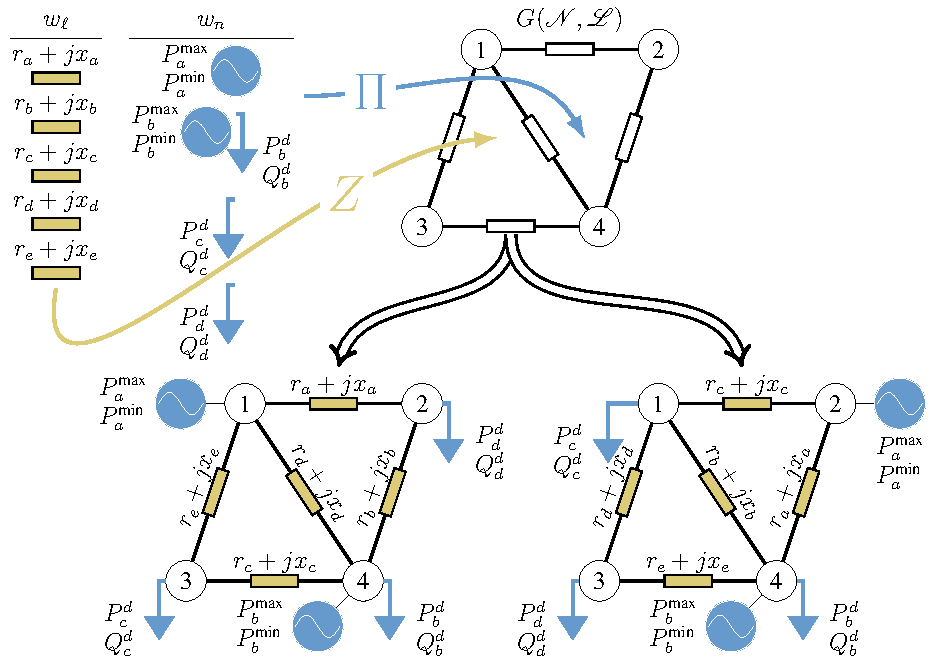
\includegraphics[width=0.6\textwidth]{figs/variationsmodecartoon.pdf}
\caption[Variations Mode Approach]{Conceptual illustration of how the \syngrid{} variations mode operates. The main computational challenge is solving for permutations $Z$ and $\Pi$.}
\label{fig:variations_mode_cartoon}
\end{figure}


%%------------------------------------------
\clearpage
\section{\syngrid{} -- Base Mode}
\label{sec:syngrid_base}


The base mode synthetic grid generation begins with the topology creation using small-world properties and realistic power grid features. The second step is bus type assignment. It utilizes a direct search procedure for the best generation, load and connection bus assignment with examining a numerical measure, called ``bus type entropy''. Once the bus types are determined, generation capacities, generation dispatch and load settings are assigned in the next step. The algorithms utilize non-trivial correlations between electric parameters to assign statistically random set of variables in each step. By providing all necessary data for DC PF study such as electric topology, generation and load settings, DC PF is executed to test the state variables including phase angle differences and flow distribution. If the created case does not pass the predefined criteria for the state variables, it will be sent to the previous modules to modify the created synthetic case. Once the generated case passed the state variables test, the transmission line capacity module determines the line capacities, based on the synthetic grid flow distributions. The module for generation cost modelling uses the generation capacities to determine the fuel types and then assigns the cost models based on them.

The \syngrid{} base mode functionality currently consists of the five components described in the sections below.


\subsection{Generation of Electrical Topology}
\label{sec:Basemode}


This module generates random grid-unique electric topologies with scalable network size featuring the same kind of small-world electrical topology of real world power transmission network. Based on the fact that in real world power grids usually a large-scale systems consist of a number of smaller-size subsystems, which are interconnected by sparse and important tie lines, \syngrid{} base mode generates the cases in a hierarchical way. First, it forms connected subnetworks with size limited by the connectivity requirements. Then connects the subnetworks through lattice connections and finally, generates the line impedances from specific distributions and assign them to the links in the topology network.

The first step to form subnetworks is to select the size of the them according to connectivity limitation. To produce a sparse but connected topology, the small-world requires $\langle k \rangle << N << e^{\langle k \rangle}$. On the other hand real-world power grids have a very low average nodal degree with $\langle k \rangle = 2 \sim 5$, regardless of the network size. Therefore, this limits the network size much smaller than 150 in order to produce a connected topology. Then, to link selection of subnetworks, a number $k$ of links at random will be selected from a local neighborhood $N_{d_0}$ ($N^i_{d_0} = \{ j; | j-i | < d_0$ for node $i$) with the distance threshold of $d_0$, where k comes from a geometric distribution. Final step to form subnetworks is link rewiring. A Markov chain with transition probabilities of  ($\alpha, \beta$) is used to select clusters of nods and therefore groups of links to be rewired and the by a specific rewiring probability $q_rw$ which is directly obtained from statistical estimates, some links will be selected to rewire. For the lattice connections, an integer number around $\langle k \rangle$ will be selected at random from neighboring subnetworks to form the whole large-scale power grid network. A number $M$ of line impedances will be generated from a heavy-trailed distributions, and then sorted by magnitude and group into local links, rewire links, and lattice connections. More details are available in~\cite{syngrid_nestedSW}.

\subsection{Bus Type Assignment}

The best set of generation, load and connection bus assignments for a given synthetic power grid will be located in this component. There exist non-trivial correlations between the three bus types and other topology metrics such as node degrees and clustering coefficients in a real-world power grid; and a random permutation of the grid's original bus type assignments will dramatically change the grid dynamics and makes the resulting network have no longer like a power grid. Therefore, the Bus Type Entropy has been defined as a numerical weighted measure to quantify and characterize the ``correlated'' bus type assignments. Two different mathematical definitions for Bus Type Entropy are as following:
\begin{equation}
	W_0(\mathbb{T}) = - \sum^3_{k=1}r_k \cdot \log(r_k) -\sum^6_{k=1}R_k \cdot \log(R_k),
\end{equation}
\begin{equation}
	W_1(\mathbb{T}) = - \sum^3_{k=1}\log(r_k) \cdot N_k -\sum^6_{k=1}\log(R_k) \cdot M_k, \end{equation}
where $r_k=\frac{N_k}{N}$ represent the bus type ratio where $r_1= \frac{N_1}{N}$ , $r_2=\frac{N_2}{N}$ and $r_3=\frac{N_3}{N}$ are the ratios of generation (G), load (L) and connection (C) buses in a grid with network size N, respectively. And $R_k=\frac{M_k}{M}$, corresponding to the link type ratio where $R_{1\_6}$ represent the ratios of the six types of branches in a grid, i.e. GG, LL, CC, GL, GC, LC, respectively, with $M_k$ being the total number of branches of a specific link type in the grid.

The best set of bus type assignments will be determine in four steps. First, the empirical PDF of randomized bus type assignments with respect to the grid size and its connecting topology will be generate to calculate the estimated fitting distribution parameters of $(\mu,\sigma)$. Then, the scaling property of normalized distance called d will be calculated using following equations
\begin{equation}
d_{W_0}(N) = \begin{cases}
		-1.721 \cdot \ln(N) + 8 & \ln(N) \leq 8 \\
		-6.003 \times 10^{-14} \cdot (\ln(N))^{15.48} & \ln(N) > 8,
		\end{cases}
\end{equation}
\begin{equation}
d_{W_1}(N) = \begin{cases}
		-1.748 \cdot \ln(N) + 8.276 & \ln(N) \leq 8 \\
		-6.053 \times 10^{-22} \cdot (\ln(N))^{24.10} & \ln(N) > 8,
		\end{cases}
\end{equation}
Once the fitting parameters and d are calculated, the target entropy value of $W^*$ can be calculate using $W^*=\mu+\sigma \cdot d_W(N)$, which is consistent with that observed in realistic grids. Finally, an optimization algorithm with objective function of
\begin{equation}
\min\limits_{\forall \mathbb{T}} \varepsilon = |W_1(\mathbb{T}) - W^* |
\end{equation}
will be implemented to search for the desired bus type assignments with respect to the $W^*$ to determine the best set of bus type assignments. More details on bus type assignment can be found in~\cite{syngrid_bustype}.

\subsection{Generation Capacities, Load  and Generation Settings}

Phases three and four generate statistically correct random set of generation capacities and loads and assign them to the generation and load buses in a synthetic grid. Algorithms are according to the estimated distribution of individual generation capacities and loads, approximated scaling function of aggregated generation capacity and load and the correlation between generation capacity and loads with nodal degree of related buses. In real-world power grids, more than $99\%$ of the generation units/loads follow an exponential distribution with about $1\%$ having extremely large capacities falling out of the normal range defined by the expected exponential distribution. Therefore, a statistically correct random set of generation capacities and load will generate based on the derived exponential distribution distributions. For both aggregate generation capacity and load the approximate scaling function can be represented as function of network size as
\begin{equation} \label{scale_pgmax}
	\log^{tot}_{g,Max}(N) = -0.21 \cdot \log(N)^2 + 2.06 \cdot \log(N) + 0.66,
\end{equation}
\begin{equation} \label{scale_pl}
	\log^{tot}_{L}(N) = -0.20 \cdot \log(N)^2 + 1.98 \cdot \log(N) + 0.58,
\end{equation}
where $P^{tot}_{g,Max}$ denotes the estimated total generation capacity, $P_L^{tot}$ denotes the estimated total demand, and the logarithm is with base 10. The generated random sets of generation capacities and loads will be checked and scaled to ensure the aggregated generation capacities and loads remain in the range specified by Eqs. \ref {scale_pgmax} and \ref{scale_pl}. The final step is to assign the generated statistically correct random sets to the related buses. There exists a non-trivial correlation between the normalized nodal degree of a generation bus and its capacity by a Pearson coefficient of $\rho(\overline{P^{Max}_{g_n}} , \overline{k_n}) \in [0.15, 0.50]$. Moreover, for the normalized node degree of load buses and their loads, the  Pearson's coefficient is $\rho (\overline {P_{L_n}} , \overline{k_n}) \in [0.30, 0.60]$. Based on these non-trivial correlations, empirical 2-D probability mass function (PMF) are extracted to use as a guidance map to assign generated random sets of generation capacities and loads based on the node degrees. Details on generation capacity and load assignment are available in~\cite{syngrid_gen_load}.

Generation dispatch is the other vital component to build a valid synthetic grid. It enables the toolkit to perform DC PF study, test the created synthetic cases, and use the calculated flow distributions to determine transmission line capacities. Our statistical studies indicate that there exist non-trivial correlation between the generation capacities and its generations dispatch as evidenced by the Pearson coefficient of $\rho(\overline{P^{Max}_{g_n}} , \overline{P_{g_n}}) \in [0.75, 0.95]$ evaluated for realistic power grid data. All the generators in the system can be divided to three categories based on their dispatch factor: I) uncommitted unites with $\alpha_g=0$, II) partially committed unites with $\alpha_g < 1$, and III) fully committed units with $\alpha_g \approx 1$. It is found that in a typical system about $10 \sim 20\%$ of generators are uncommitted with small and medium generation capacity and about $40 \sim 50\%$ of the generators belong to category II. There exist a significant correlation between the normalized generation capacities and their dispatch factor ($\alpha=\frac{P_g}{P_g^{max}}$) with a Pearson coefficient $\rho(\overline{P^{Max}_{g_n}} , \overline{\alpha_n}) \in [0.15, 0.55]$ in realistic power grids. Therefore, we can extract 2-D PMF for the given reference realistic grid. To reproduce a similar correlation between the generation dispatch and the generation capacity as found in real grid systems, we formulate a 2-D table based on 2-D empirical PMF and assign dispatch factors to each generation bus based on generation capacities and 2-D PMF table.

The next step is to generate statistically correct random set of dispatch factors. We found that for realistic power grids, more than 99\% of the committed generations have capacities following an exponential distribution with about 1\% having extremely large capacities falling outside of the normal range defined by expected exponential distribution indicated by imperial probability density function (PDF) committed unites.
Given a synthetic grid topology with N buses and determined generation capacities and load settings, the algorithm selects a randomly correct set of generation capacities for both committed and uncommitted units which follows 99\% rule for committed unites and uniform distribution for uncommitted unites. Next by generating statistically correct random set of dispatch factors, it assigns them to the selected generation capacities in generation buses based on obtained statistical pattern.

Given a synthetic grid topology with N buses and determined generation capacities and load settings, the algorithm selects a randomly correct set of generation capacities for both committed and uncommitted units which follows $99\%$ rule for committed unites and uniform distribution for uncommitted unites. Next by generating statistically correct random set of dispatch factors, it assigns them to the selected generation capacities in generation buses based on a 2-D empirical PMF of normalized generation capacities and dispatch factors. More details are available in~\cite{syngrid_transmissionline}.

\subsection{Transmission Line Capacity}

Our initial experiments on statistical distribution of transmission gauge ratio show that the best distribution, which fits the distribution of transmission gauge ratios $\beta_l =\frac{F_l}{F^{Max}_l}$ is exponential distribution. The statistics collected from realistic grids also indicate that there exists a considerable correlation between the transmission gauge ratio and its flow distribution. The Pearson's coefficient varies in range of 0.35 – 0.65. Studying correlation between transmission gauge ratio and normalized flow distribution, we may extract an empirical 2-D PMF and based on that a 2-D PMF table can be formulated to enable an algorithm to assign transmission line capacities to the synthetic power grid. It is worthy to note that in power systems, three different capacities define for transmission lines i.e. long term, short term, and emergency capacity and in this study, we focus on long-term capacity of transmission lines. The transmission line capacities will be determined in three steps. First, a statistically correct random set of transmission gauge ratios will be generated; and using derived 2-D probability distribution table, the transmission gauge ratios will be assigned to each transmission line with respect to the grid flow distribution calculated from the DC power flow solution. More details are available in~\cite{syngrid_transmissionline}.

\subsection{Generation Cost Function}

The essential component to perform energy economic studies, such as OPF problem, is to determine generator cost models and their associated coefficients. The algorithm utilizes the statistical analysis of actual grids and available information on generation units to determine fuel types and generation cost models based on pre-determined generation capacities.

The generation mix of U.S. Energy Information Association data  is studied to proposed the fuel type assignment algorithm. For simplicity, all different technologies/fuel types in the generation mix are combined into five major categories of Hydro, Wind, Natural Gas, Coal, and Nuclear to avoid relatively complicated modeling for very small portion of total installed generation capacity. Statistical analysis on power plants for all the three North American electric power interconnections shows that there exist a strong correlation between normalized generation capacities of power plants and their discretized fuel types by a Pearson coefficient of $\rho(\overline{P^{Max}_{g_n}}, \overline{TP_n}) \in [0.75, 0.95]$. Given a data set of generation unit capacity and discretized fuel types, we may define a joint distribution function in the two-dimensional space of $(\overline{P^{Max}_{g_n}}, \overline{TP_n})$. The 2-D density function $f(\overline{P^{Max}_{g_n}}, \overline{TP_n})$, when integrated over a set S gives the probability that $(\overline{P^{Max}_{g_n}}, \overline{TP_n})$ falls into the set:

\begin{equation}
	\Pr(A) = \Pr\{ (\overline{P^{Max}_{g_n}} , \overline{TP_n}) \in S \},
\end{equation}
Thus, the 2-D empirical probability mass function (PMF) cab be extracted to use as a guidance map to assign fuel types to generators based on their normalized generation capacity. Figure 2 shows imperial 2-D PMF of normalized generation capacity versus discretized fuel types for EI system. Once the fuel types determined, generation cost models will be assigned accordingly. For the generation cost model, we consider two approaches to assign no load and production cost to each generator:
\begin{equation}
	\textrm{Approach }A : c(p) = a_0 + c_f(b_1P+b_2P^2),
\end{equation}
\begin{equation}
	\textrm{Approach }B : c(p) = a_0 + a_1P+a_2P^2
\end{equation}
where $\{a_i \colon i=0,1,2\}$ and $\{b_i \colon i=1,2\}$ indicate the fuel-dependent cost model coefficients, c\_f refers to fuel cost and P is generator output.
The approa A utilizes average heat rates of power plants and their fuel costs obtained from EIA data, to model cost functions. On the other hand, A models the generation cost based on the dispatch cost coefficients derived from generation block-offer schedule data of ISO-NE  and PJM differentiated by fuel type. No load costs for wind and hydro power plants are set to zero. The cost coefficients data summarized in Table \ref{tab_coa} and \ref{tab_cob} are used to assign for each generator by its fuel type and capacity.

\begin{table}
\centering
\begin{threeparttable}
\caption{Coefficients Approach 1}
\label{tab_coa}
\footnotesize
\begin{tabular}{l c c c c c p{0.50\linewidth}}
\toprule
% Fuel Type   & Capacity(MW) & $a_0$ (\$/h) & $c_f$ (\$/MBtu) & $b_1$ (MBtu/MWh) & $b_2$ (MBtu/MWh$^2$) \\
Fuel Type & Capacity & $a_0$  & $c_f$     & $b_1$      & $b_2$ \\
          & (MW)     & (\$/h) & (\$/MBtu) & (MBtu/MWh) & (MBtu/MWh$^2$) \\
\midrule
Coal      & 0 - 75      & 0 - 238      & 2.16   & 9.43-18.53    & 0  \\
Coal      & 75 - 150    & 238 - 745    & 2.16   & 9.43-18.53    & 0 \\
Coal      & 150 - 350   & 745 - 1213   & 2.16   & 9.43-18.53    & 0  \\
Coal      & 0 \textgreater 350   & 1213 - 3043      & 2.16   & 9.43-18.53    & 0 \\
Natural Gas       & 0 - 400  & 0 - 600      &  2.59    & 6.5 - 17.5    & 0 \\
Natural Gas       & 0 \textgreater 400    & 600 - 3859   &  2.59   & 6.5 - 17.5     & 0 \\
Nuclear           & - - -    & 1000 - 1500  &  0.85   & 10.46          & 0      \\
Hydro/Wind        & - - -    & 0            &  0      & 0              & 0      \\
\bottomrule
\end{tabular}
\end{threeparttable}
\end{table}

\begin{table}
\centering
\begin{threeparttable}
\caption{Coefficients Approach 2}
\label{tab_cob}
\footnotesize
\begin{tabular}{l c c c c p{0.50\linewidth}}
\toprule
% Fuel Type   & Capacity(MW) & $a_0$ (\$ / h) & $a_1$ (\$ / MWh) & $a_2$ (\$ / MWh$^2$) \\
Fuel Type & Capacity & $a_0$  & $a_1$    & $a_2$ \\
          & (MW)     & (\$/h) & (\$/MWh) & (\$/MWh$^2$) \\
\midrule
Coal      & 0 - 75     & 0 - 238       & 19   & 0.001   \\
Coal      & 75 - 150   & 238 - 745     & 19   & 0.001  \\
Coal      & 150 - 35   & 745 - 1213    & 19   & 0.001   \\
Coal      & 0 \textgreater 350      & 1213 - 3043   & 19   & 0.001  \\
Natural Gas       & 0 - 400   & 0 - 238      & 23.13 - 57.03   & 0.002 - 0.008  \\
Natural Gas       & 0 \textgreater 400     & 0 - 238      & 23.13 - 57.03   & 0.002 - 0.008   \\
Nuclear               & - - -     & 1000 - 1500  & 5 - 11          & 0.00015 - 0.00023        \\
Hydro/Wind              & - - -     & 0            & 0               & 0      \\
\bottomrule
\end{tabular}
\end{threeparttable}
\end{table}



%%------------------------------------------
\clearpage
\section{\syngrid{} -- Variations Mode}
\label{sec:syngrid_vm}
Figure~\ref{fig:syngrid_flowchart} provides a flowchart of the variations mode operation.
The following subsections describe the algorithms implemented in each of the subprocesses.
	
\begin{figure}
\centering
\resizebox{0.9\textwidth}{!}{
%\documentclass{standalone}
%\standaloneconfig{border=1pt}
%
%\usepackage{tikz}                  % load graphics drawing packgate tikz
%\usetikzlibrary{graphs,arrows.meta,decorations.pathreplacing,intersections,positioning,calc}
%\usetikzlibrary{datavisualization.formats.functions,datavisualization,shapes.geometric}
%\usepackage{amsmath}

%\begin{document}

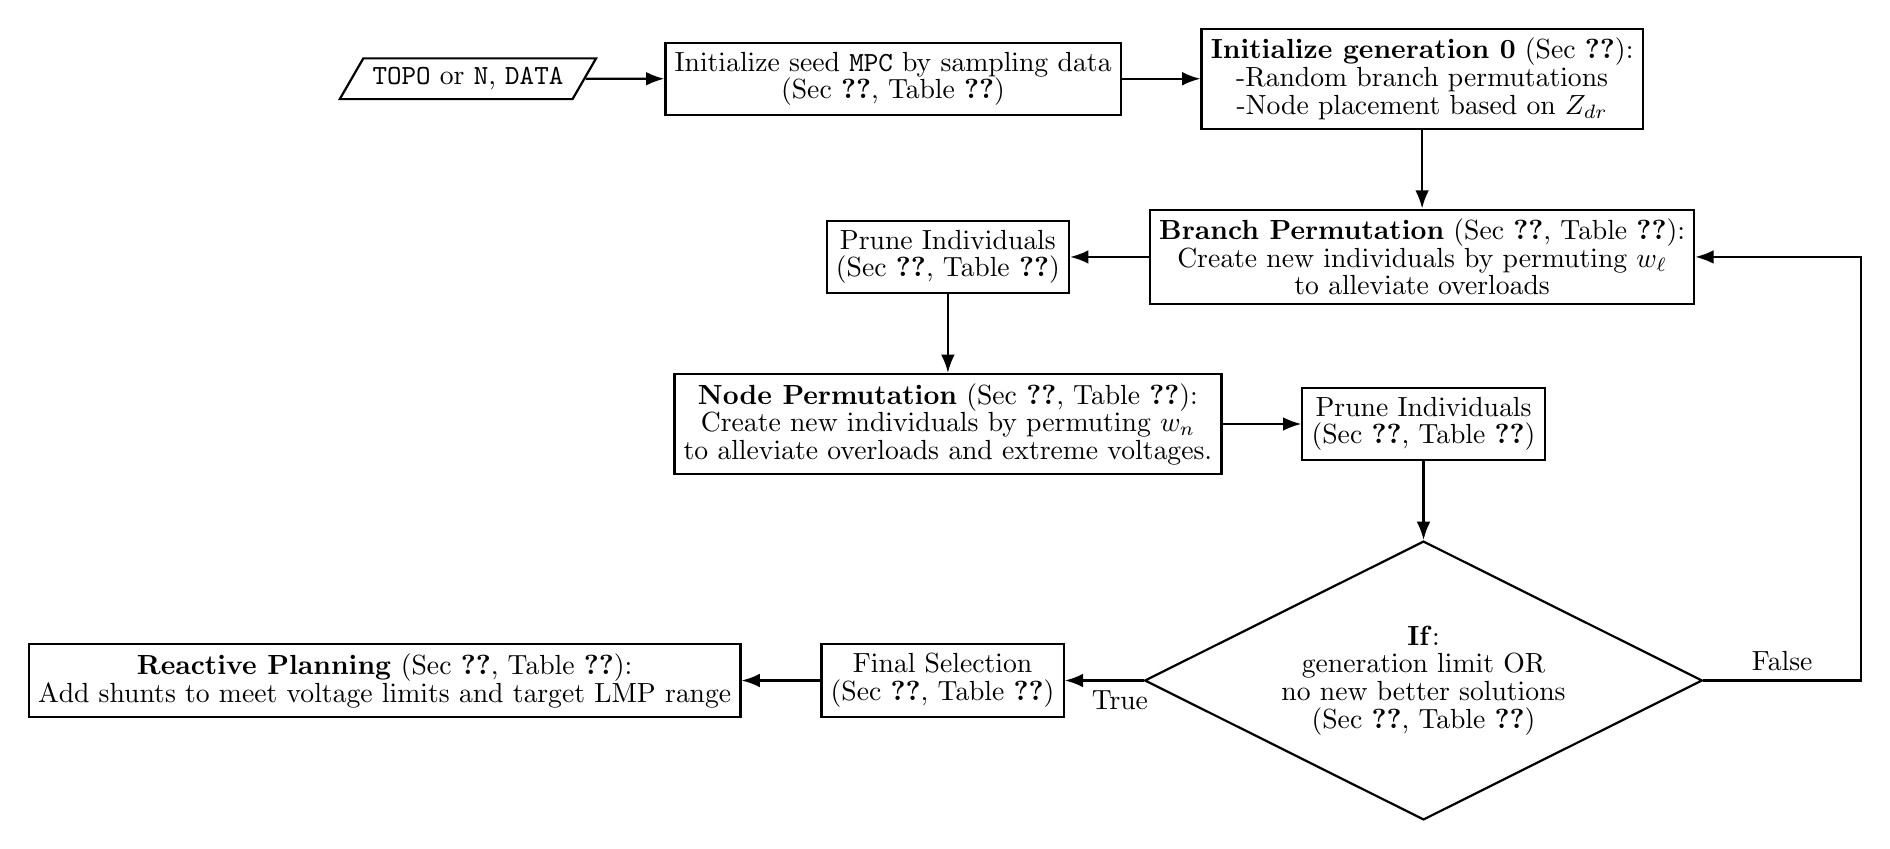
\begin{tikzpicture}[%
    thick,
    >={Latex},
    input/.style={trapezium,draw=black, text=black,trapezium left angle=60, trapezium right angle=120, align=center},
    process/.style={rectangle, draw=black, text=black, align=center, execute at begin node=\setlength{\baselineskip}{1em}},
    start/.style={ellipse,draw=black, text=black},
    decision/.style={diamond, aspect=2, draw=black, text=black, align=center, execute at begin node=\setlength{\baselineskip}{1em}}
    ]

\node[input] (input) {\texttt{TOPO} or \texttt{N}, \texttt{DATA}};
\node[process, right=of input] (samp) {Initialize seed \texttt{MPC} by sampling data\\ (Sec~\ref{sec:vm_smpl}, Table~\ref{tab:smplopt})};
\node[process, right=of samp] (init) {\textbf{Initialize generation 0} (Sec~\ref{sec:vm_init}):\\ -Random branch permutations \\ -Node placement based on $Z_{dr}$};
\node[process, below=of init] (branch) {\textbf{Branch Permutation} (Sec~\ref{sec:vm_branch}, Table~\ref{tab:branchpermopt}):\\ Create new individuals by permuting $w_{\ell}$\\ to alleviate overloads};
\node[process, left=of branch] (selection_b) {Prune Individuals\\(Sec~\ref{sec:vm_ea}, Table~\ref{tab:eaopt})};
\node[process, below=of selection_b] (node) {\textbf{Node Permutation} (Sec~\ref{sec:vm_node}, Table~\ref{tab:nodepermopt}):\\ Create new individuals by permuting $w_{n}$\\ to alleviate overloads and extreme voltages.};
\node[process, right=of node] (selection_n) {Prune Individuals\\(Sec~\ref{sec:vm_ea}, Table~\ref{tab:eaopt})};
\node[decision, below=of selection_n] (loop) {\textbf{If}:\\ generation limit OR \\ no new better solutions \\ (Sec~\ref{sec:vm_ea}, Table~\ref{tab:eaopt})};
\node[process, left=of loop] (selection_f) {Final Selection\\(Sec~\ref{sec:vm_ea}, Table~\ref{tab:eaopt})};
\node[process, left=of selection_f] (shunts) {\textbf{Reactive Planning} (Sec~\ref{sec:vm_shunts}, Table~\ref{tab:shuntsopt}): \\ Add shunts to meet voltage limits and target LMP range};

\draw[->] (input) -- (samp);
\draw[->] (samp) -- (init);
\draw[->] (init) -- (branch);
\draw[->] (branch) -- (selection_b);
\draw[->] (selection_b) -- (node);
\draw[->] (node) -- (selection_n);
\draw[->] (selection_n) -- (loop);
\draw[->] (loop) -- node[pos=0.3][auto]{True} (selection_f);
\draw[->] (selection_f) -- (shunts);
\draw[->] (loop.east) -- node[auto]{False} +(2cm, 0) |- (branch);

\end{tikzpicture}

%\end{document}}
\caption{Variations Mode Flowchart}
\label{fig:syngrid_flowchart}
\end{figure}

%% ----------- Creating Seed Data ----------------------------------
\subsection{Creating Seed Data}\label{sec:vm_smpl}
As illustrated in Figure~\ref{fig:variations_mode_cartoon} there are two main categories to sample: branch and node properties.
\subsubsection{Branch Properties}
If the \codeq{direct} method of sampling is selected then elements are picked uniformly at random from the list provided in the \code{data} input struct.
When the \codeq{kde} method is selected the process proceeds in three steps.

First, the number of transformers is estimated as:
\begin{equation}
	n_{x} = \text{round}\left[n_l \times \frac{n^s_x}{n^s_l} \right],
\end{equation}
where $n^s_x$ is the number of  transformers in the \code{data} struct, $n^s_l$ the total number of branches in the seed \code{data} struct. 
The total branch and transformer samples needed are $n_l$ and $n_x$. 
For example, there could be 3000 branch samples in the \code{data} struct ($n^s_l=3000$), however, the \code{topo} input calls for only 1000 samples ($n_l=1000$) to be created.

In the second step a KDE is fit to all branches that are \emph{not} transformers.
The $n_l - n_x$ lines are then sampled from the KDE.
Finally, another KDE is fit to all the transformers in \code{data}, and sampled $n_x$ times.

\subsubsection{Bus Properties}
The bus properties are somewhat more complicated since both load and generation are needed.
Load values can be either sampled directly or using a KDE in a method quite similar to the previous section.
Generation values are always sampled directly following the load sampling.

The basic idea is that there are a few different types of configurations are considered:
\begin{itemize}
	\item Buses with no load and no generation
	\item Buses with no load and generation
	\item Buses with both load and generation
	\item Buses with load only
\end{itemize}
The number of buses with generators is either calculated based on the ratio in the input data \emph{or} specified directly by the user via the \code{ngbuses} option.
Similarly for the number of no load buses.
The number of no load, no generation buses is chosen uniformly at random as between 0.6 and 0.95 of the number of no load buses. 
With these numbers, the rest of can be trivially derived. 

The one additional consideration is regarding number of generators on a bus.
If the generator bus is specified in the input data it is used to group generator sets and thus multiple ones can be sampled at once.

Finally, the ratio between generation capacity and load is considered. 
This is calculated directly from the input data when \code{usegen2load=1} (default).
If \code{usegen2load=0} then the ratio is sampled uniformly at random between 1.3 and 1.6.
Single generators are resampled randomly to try and shift the ratio towards the desired goal. 
If the \codeq{direct} sampling method is used, individual loads will also be resampled.

%% ----------- Initial Permuation -------------------------------------
\subsection{Initial Permutation} \label{sec:vm_init}
Initial permutation of branch parameters is done uniformly at random.
The initial node permutation leverages observations in \cite{schweitzer2016GOTF} correlating generators and the driving point impedances, $Z_{\text{dr}}$ at their bus.
In general generators appear to be located at buses with \emph{larger} magnitude $Z_{\text{dr}}$.
Within generator buses, however, \emph{larger} generators are paired with \emph{smaller} $Z_{\text{dr}}$.

To select generator buses, the driving point impedances are ordered in descending order $|Z_{\text{dr}}^1| \geq |Z_{\text{dr}}^2| \geq \ldots \geq |Z_{\text{dr}}^{n_b}|$.
The fact that the order statistics of the Uniform distribution are distributed as $\text{Beta}(k, n-k + 1)$, with $n$ the number of samples, is used to sample buses ``around'' a certain range in the order $Z_{\text{dr}}$ values.
If $n=n_b$, the distribution quickly becomes far too narrow. 
Therefore $n=10$ is fixed and the resulting samples are scaled.
Specifically, the $\text{Beta}(8,3)$ distribution is sampled $n_g$ times.
Each sample, $s\in[0,1]$ maps to an index $i$ as:
\begin{equation}
	i = \text{round}(s\times n_b).
\end{equation}
In this way $n_g$ indices are selected that are scattered more heavily towards larger $Z_{\text{dr}}$ values.

Generators are assigned to the selected buses with negative correlation, so that  the largest generator gets the smallest $Z_{\text{dr}}$. 
Finally, 10\% of the generators are randomly selected and swapped with another randomly selected generator to add some noise and avoid perfect negative correlation.

%% ----------- Evolutionary Algorithm Loop -----------------------
\subsection{Evolutionary Algorithm Loop} \label{sec:vm_ea}
The main loop of the variations mode is an Evolutionary Algorithm (EA) inspired procedure.
Each loop is referred to as a generation, and each generation is composed of several individuals.
Individuals in this case are simply \matpower{} cases with different permutations of sets $w_{\ell}$ and $w_{n}$.

The ``evolution'' refers to the fact that in each an individual produces a new individual, i.e. \matpower{} case, by permuting some of its properties to achieve some objective.
Branch and node properties are handled separately, and those procedures are described in the subsequent sections.
Finally, each permutation block can be iterated several times, increasing the number of cases that can be permuted.
This is illustrated in Figure~\ref{fig:example_evolution} for the case where both branch and node permutations are performed twice.
As such, each generation is in a sense comprised of a few `sub-generations'.
To avoid a dimensional explosion of cases, pruning procedures reduce the number of progenitors (i.e. potential parents) that are passed between permutations blocks.

\begin{figure}
\centering
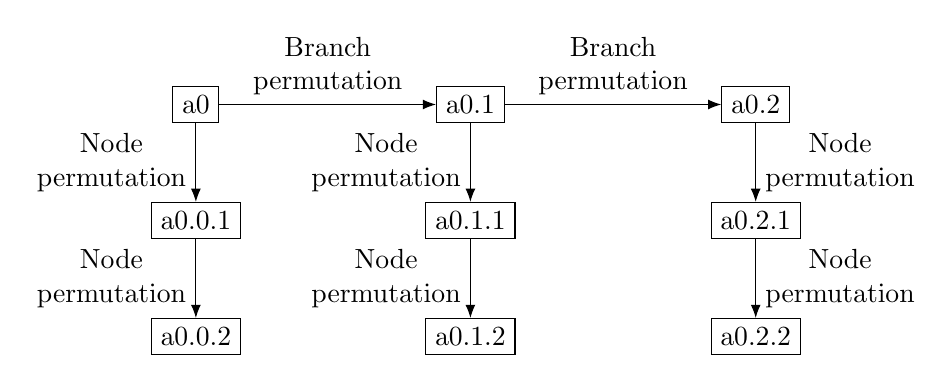
\begin{tikzpicture}
	\node[draw, align=center] (a0) {a0};
	\node[right=2.75cm of a0, draw, align=center] (a01) {a0.1};
	\node[right=2.75cm of a01, draw, align=center] (a02) {a0.2};
	
	\node[draw, below=of a0] (a001) {a0.0.1};
	\node[draw, below=of a001] (a002) {a0.0.2};
	
	\node[draw, below=of a01] (a011) {a0.1.1};
	\node[draw, below=of a011] (a012) {a0.1.2};
	
	\node[draw, below=of a02] (a021) {a0.2.1};
	\node[draw, below=of a021] (a022) {a0.2.2};
	
	\draw[-{Latex}] (a0) -- node[align=center, above] {Branch\\ permutation} (a01);
	\draw[-{Latex}] (a01) -- node[align=center, above] {Branch\\ permutation} (a02);
	
	\draw[-{Latex}] (a0) -- node[align=center, left] {Node\\ permutation} (a001);
	\draw[-{Latex}] (a001) -- node[align=center, left] {Node\\ permutation} (a002);
	
	\draw[-{Latex}] (a01) -- node[align=center, left] {Node\\ permutation} (a011);
	\draw[-{Latex}] (a011) -- node[align=center, left] {Node\\ permutation} (a012);
	
	\draw[-{Latex}] (a02) -- node[align=center, right] {Node\\ permutation} (a021);
	\draw[-{Latex}] (a021) -- node[align=center, right] {Node\\ permutation} (a022);
\end{tikzpicture}
\caption{Example evolutions from a single parent node `a0' when both branch and node permutations are performed twice.}
\label{fig:example_evolution}
 \end{figure}
 
%% ----------- BranchPermuation -----------------------------------
\subsection{Branch Permutation} \label{sec:vm_branch}
\subsubsection{General Formulation}
The branch permutation problem can be though of as a search for permutation $Z$ of the branch ratings $F_{\text{max}}$ and impedances ($r_s$ and $x_s$), that would minimize overload flows.
In the formulation, flows $f$ are assumed to remain constant.
While this is clearly not the case, by minimizing the difference between the old and new impedances, flows are encouraged to remain similar.
The problem can be formulated as:
\begin{equation}
\begin{aligned}
\underset{ t, t_r, t_x, Z}{\text{\bfseries Minimize}} \quad & \mathbf{1}^T  (t + t_r + t_x)\\
\text{\bfseries Subject to} \quad & t + (Z F_{\text{max}} - f) \geq 0 \\
						& - t_r \leq Z r_s - r_s \leq t_r \\
						& - t_x \leq Z x_s - x_s \leq t_x \\
						&Z \mathbf{1} = \mathbf{1},; \mathbf{1}^T Z= \mathbf{1}^T \\
						& t, t_r, t_x \geq 0 \\
						&Z\in\{0,1\}
\end{aligned}
\end{equation}
Constraint $t + (ZF_{\text{max}} - f) \geq 0$ in conjunction with $t \geq 0$ forces $t_i$ to be the difference between flow and rating, if $f_i$ is greater than rating $[ZF_{\text{max}}]_i$, and thus discourages overloads.
The constraints with $r_s$ and $x_s$ penalize deviation from the original (non-permuted) impedance, and the following constraint forces $Z$ to be a permutation matrix, that is, doubly stochastic and binary valued.

Unfortunately, this problem suffers greatly from dimensionality, since $Z$ is an $n_l \times n_l$ matrix.
Therefore, the algorithm in the \syngrid{} implementation uses a simplified greedy approach to solve for $Z$.
It is important to note that since a greedy approach is used, optimality (even improvement) is not guaranteed.

\subsubsection{Simplified Approach}
First, the set $\mathcal{B}$ of all overloaded branches that require attention is identified:
\begin{equation}
	\mathcal{B} = \left\{i: \frac{|f_i|}{F^i_{\text{max}}} > x \quad \forall i \in \mathcal{I}_l\right\},
\end{equation}
where $f_i$ and $F^i_{\text{max}}$ are the flow and rating of branch $i$, and $x$ is an acceptable ratio.
Initially $x$ might be 1 to find only truly overloaded branches.
However, it can be useful to allow $x$ to dip below 1, which has the effect of seeking capacity margins on all the branches.

For each element $i\in\mathcal{B}$ there is a candidate set $\mathcal{C}_i$ of possible branches with which to swap properties,
\begin{equation}
	\mathcal{C}_i = \left\{j: F_{\text{max}}^j x\geq |f_i|, |f_j| \leq F^i_{\text{max}} x \quad \forall i \in \mathcal{I}_l\right\}.
\end{equation}
That is, the set of branches whose ratings are \emph{large} enough to support the flow on branch $i$, and whose flows are \emph{small} enough to be supported by branch $i$'s rating.

The remaining task is to select one candidate, $j^{\star}$, out of $\mathcal{C}_i$ to swap with branch $i$.
Three tests are used to determine the quality of each candidate:
\begin{description}
\item[Impedance Test] Measures the distance between the impedance of each branch ${j\in\mathcal{C}_{i}}$ and $i$:
\begin{equation}
	z_{i}(j) = (r^j_s - r^i_s)^2 + (x^j_s - x^i_s)^2.
\end{equation}
\item[Rating Test A] Seeks the largest margin between the flow on branch $i$ and the ratings on branches ${j\in\mathcal{C}_{i}}$:
\begin{equation}
	m^a_{i}(j) = |f_i| - F_{\text{max}}^j
\end{equation} 
\item[Rating Test B] Seeks the largest margin between the flow on each branch ${j\in\mathcal{C}_{i}}$ and the rating of branch $i$:
\begin{equation}
	m^b_{i}(j) = |f_{j}| - F_{\text{max}}^i
\end{equation}
\end{description}
Lower values for all three tests are desirable and therefore, the final selection can be formalized as:
\begin{equation}
	j^{\star} = \argmin_{j\in\mathcal{C}_{i}} w_z(j) z_{i}(j) + w_a(j) m^a_{i}(j) + w_b(j) m^b_{i}(j),
\end{equation}
where $w_z$, $w_a$, and $w_b$ are used to weights to the different tests.

Letting $\text{ord}_t(j)$ return the order statistic of element $j\in\mathcal{C}_{i}$ for test $t$, so that if $t(j)$ is the smallest $\text{ord}_t(j) = 1$, second smallest $\text{ord}(j)=2$ etc., then the implemented weighting scheme is:
\begin{equation}
	w_z(j) = \frac{\text{ord}_{z_{i}}(j)}{z_{i}(j)},
\end{equation}
and similarly for $w_a(j)$ and $w_b(j)$.

%% ----------- Node Permutation -----------------------------------
\subsection{Node Permutation} \label{sec:vm_node}
The node permutation problem is solved in two steps:
\begin{enumerate}
	\item A desired injection change, $\Delta P$ and $\Delta Q$ is sought, which, given several assumptions, should minimize overloads and stabilize the voltage profile.
	\item A permutation vector $\pi$ is sought that best achieves the desired change in injection calculated in Step 1.
\end{enumerate}

\subsubsection{Desired Injection Change}
Bus and branch effects of changing injections, $\Delta P$ and $\Delta Q$, are captures by linearizing the power flow around the given operating point. 
Voltage effects are related via the columns of the system Jacobian associated with the voltage magnitude,
\begin{equation}
	\begin{pmatrix} \Delta P \\ \Delta Q \end{pmatrix} = J_v \Delta v,
\end{equation}
and the branch flow effects are captured using AC-PTDFs,
\begin{equation}
	\begin{pmatrix} \Delta P_f \\ \Delta Q_f \end{pmatrix} = H_f \begin{pmatrix} \Delta P \\ \Delta Q \end{pmatrix},
\end{equation}
where $ \Delta v$, is the change in voltage magnitude, and $\Delta P_f$ and $\Delta Q_f$ are changes in real and reactive line flows\footnote{
For simplicity only flows at the \emph{from} end are used in the following}.

To create linear constraints on branch flows, the angle of flow on line $i\in\mathcal{I}_l$,
\begin{equation}
	\alpha_i = \begin{cases} 
		\arctan\left(\frac{Q_f^{i}}{P_f^{i}}\right) & P_f^{i} \geq 0 \\
		\pi - \arctan\left(\frac{Q_f^{i}}{P_f^{i}}\right) & P_f^{i} < 0,
		\end{cases}
\end{equation}
is considered.
New flows are only allowed to vary inside the box defined by the intersection points of the rays with angle $\alpha_i$ and $-\alpha_i$ and the limit circle of radius $r_{i}$ as shown in Figure~\ref{fig:limit_circle}.
The effective limits are thus,
\begin{equation}
	P_{f,\text{max}}^{i}= r_{i}\cos(\alpha_{i}), \quad Q_{f,\text{max}}^{i} = r_{i}\sin(\alpha_{i}).
\end{equation}
With, $P_{f,0}$, $Q_{f,0}$, and $v_0$ as the initial real and reactive flows, and voltage magnitude, the desired injection  change is formulated as the solution to:
\begin{subequations}
\begin{align}
\underset{\Delta P, \Delta Q, \Delta v}{\text{\bfseries Minimize}} \quad  & \| \Delta P \|_1 + \| \Delta Q \|_1 + w_p^Ts_p + w_q^Ts_q + w_v\cdot s_v \\
\text{\bfseries Subject to} \quad & \begin{pmatrix} \Delta P \\ \Delta Q \end{pmatrix} - J_v \Delta v = 0\\ 
 						& v_{\text{min}} - v_0 - s_v \leq \Delta v \leq v_{\text{max}} - v_0 + s_v \\
						&-\begin{pmatrix} P_{f,\text{max}} + s_p \\ Q_{f,\text{max}} + s_q \end{pmatrix}\leq \begin{pmatrix} P_{f,0} \\ Q_{f,0} \end{pmatrix} + H_f \begin{pmatrix} \Delta P \\ \Delta Q \end{pmatrix} \leq \begin{pmatrix} P_{f,\text{max}} + s_p \\ Q_{f,\text{max}} + s_q \end{pmatrix} \\
						& \mathbf{1}^T \Delta P = 0, \quad \mathbf{1}^T \Delta Q = 0 \label{eq:delta_inj_sum0}\\
						& -\Delta P_{\text{max}}\leq \Delta P \leq \Delta P_{\text{max}}, \quad -\Delta Q_{\text{max}}\leq \Delta Q \leq \Delta Q_{\text{max}} \label{eq:delta_inj_max}
\end{align}
\end{subequations}
Constraint \eqref{eq:delta_inj_sum0} forces the net change to be zero, since in the end a permutation is sought, and the limits in \eqref{eq:delta_inj_max} are simply the range of the initial injections vector. 
Additionally, slack variables are added to allow feasibility even in the event that some violations cannot be avoided.

\begin{figure}
\centering
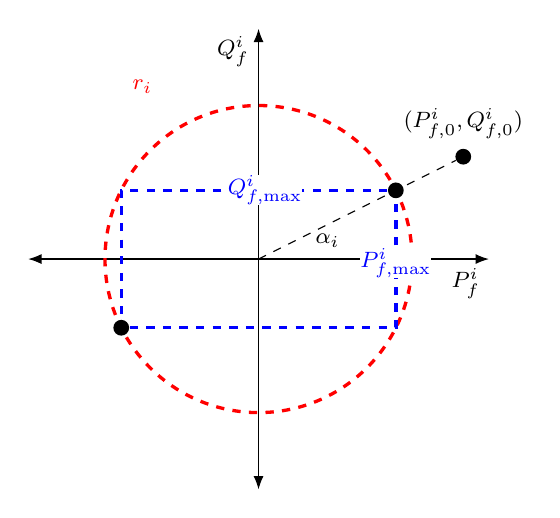
\begin{tikzpicture}[scale=1.3, font=\footnotesize]
	\draw[thin, {Latex}-{Latex}] (-2.25,0) -- (2.25,0) node[pos=0.95,below] {$P_f^{i}$};
	\draw[thin, {Latex}-{Latex}] (0,-2.25) -- (0,2.25) node[pos=0.95,left] {$Q_f^{i}$};
	
	\draw[very thick,red,dashed, name path=c] (0,0) circle[radius=1.5];
	\node[red,xshift=-5mm, yshift=5mm] at ($1.5*cos(120)*(1,0) + 1.5*sin(120)*(0,1)$) {$r_{i}$};
	
	\node[circle,fill=black,inner sep=0pt, minimum width=2mm,label={above:$(P_{f,0}^i, Q_{f,0}^{i})$}] (p0) at (2 ,1) {};
	\draw[name path=r, dashed] (0,0) --  node[pos=0.35,below] {$\alpha_{i}$} (p0);
	\path[name intersections={of=r and c, name=i}];
	\node[circle,fill=black,inner sep=0pt, minimum width=2mm] (p1) at (i-1) {}; 
	\node[circle,fill=black,inner sep=0pt, minimum width=2mm] (p2) at ($(0,0) - (i-1)$) {};
	\draw[dashed, very thick, blue] (p1) -| node[inner sep=0pt, pos=0.23,fill=white] {$Q_{f,\text{max}}^{i}$} (p2) -| node[inner sep=0pt, pos=0.75, fill=white]  {$P_{f,\text{max}}^{i}$} (p1) -- cycle;
\end{tikzpicture}
\caption[Node Permutation Line Limits]{Geometrical depiction of how line limits are set during the node permutation procedure.}
\label{fig:limit_circle}
\end{figure}


Finally, the desired new nodal injections, $P^{\star}$ and $Q^{\star}$ are defined as:
\begin{equation}
	\begin{pmatrix} P^{\star} \\ Q^{\star} \end{pmatrix}  \triangleq \begin{pmatrix} P_0 \\ Q_0 \end{pmatrix} + \begin{pmatrix} \Delta P \\ \Delta Q \end{pmatrix},
\end{equation}
where, $P_0$ and $Q_0$ are the initial injection vectors.
The next section seeks a permutation to achieve the desired injections.



\subsubsection{Greedy Permutation Approach}
The ``errors'' in real and reactive injection are defined as,
\begin{equation}
\begin{aligned}
	\epsilon_p &= P^{\star} - P_0 \\
	\epsilon_q &= Q^{\star} - Q_0,
\end{aligned}
\end{equation}
and the total magnitude error is,
\begin{equation}
	\epsilon = \sqrt{ \epsilon_p^2 - \epsilon_q^2}.
\end{equation}
The greedy node permutation approach fixes each error sequentially, beginning with the largest.
That is, vectors $P^{\star}$, $P_0$, $Q^{\star}$, and $Q_0$ are sorted such that $\epsilon_1 \geq \epsilon_2 \geq \ldots \geq \epsilon_{n_b}$.
Algorithm~\ref{alg:greedy_node_perm} returns the desired permutation vector $\pi$.
Iterating over all buses, the nearest injection to the desired injection at bus $i$ is found in set $x$.
The selected bus is then removed from the set so that the final result will be a true permutation.

\begin{algorithm}
\caption[Greedy Node Permutation]{Greedy Node Permutation}
\label{alg:greedy_node_perm}
\begin{algorithmic}
\Procedure{Greedy Node Permute}{$P^{\star}$, $P_0$, $Q^{\star}$, $Q_0$}
\State $ x \gets \{ 1,2,\ldots, n_b\}$
\For{$i \in \{1,2,\ldots, n_b\} $}
	\State $\pi(i) \gets \argmin_{j\in x} |P^{\star,i} - P_0^j| +  |Q^{\star,i} - Q_0^j| $
	\State $ x \gets x\setminus\{\pi(i)\} $
\EndFor
\State \textbf{return} {$\pi$}
\EndProcedure
\end{algorithmic}
\end{algorithm}

%% ----------- Reactive Planning -----------------------------------
\subsection{Reactive Planning} \label{sec:vm_shunts}
The basic reactive planning approach adopted is similar conceptually to {\cite{birchfield2018Power}} but leverages the OPF framework with soft limit capabilities. % \cite{birchfield2018Power}
Generator with limits equal to zero are added to each bus, with soft limits enabled. 
Since the soft limits are expensive, they will be non-zero only when necessary to satisfy the voltage constraints.
Once a solution is found, the desired shunt to add to node $i$ is:
\begin{equation}
	B_{sh}^i = \frac{s_{\text{qmax}}^i - s_{\text{qmin}}^i}{|v_i|^2},
\end{equation}
where $s_{\text{qmax}}^i$ and $s_{\text{qmin}}^i$ are violations in the positive and negative directions, respectively, of the soft limit.
Note that if the units on $s_{\text{qmax}}^i$ and $s_{\text{qmin}}^i$ are MVAr, and $v_i$ is in per-unit, then $B_{sh}^i$ will be in MVAr, which is the required format for \matpower{}.

It is additionally possible to place an upper bound on the soft limits, so that the magnitude of the shunts will be limited.
Furthermore, to ensure that no shunt is unreasonably small, all shunts with magnitudes greater than zero but smaller than a given threshold, \code{tmag}, are set to that threshold:
\begin{equation}
	B_{sh}^i = \begin{cases} B_{sh}^i & (|B_{sh}^i| \geq \code{tmag}) \cup (B_{sh}^i = 0) \\  \text{sgn}(B_{sh}^i) \cdot \code{tmag} & 0 < |B_{sh}^i| < \code{tmag}. \end{cases}
\end{equation}

%%------------------------------------------
\clearpage
\section{\tt syngrid}
\label{sec:syngrid}

The functionality of \syngrid{} is implemented using the \code{syngrid} function, with an extremely simple interface. For base mode operations, the \code{syngrid} function takes a single required input argument, the number \code{N} of desired buses in the case. It returns a standard \matpower{} case struct containing the synthetic case that was created.
\begin{Code}
>> mpc = syngrid(N);
\end{Code}

Two additional optional input arguments may be used to specify a set of \syngrid{} options (\code{sgopt}) and the name (\code{fname}) of a file to which the resulting \matpower{} case should be saved.
\begin{Code}
>> mpc = syngrid(N, sgopt);
>> mpc = syngrid(N, sgopt, fname);
\end{Code}


The variations mode, on the other hand, returns a cell array of \matpower{} cases, and requires that the user provide both an existing topology and the data to be sampled and placed on that topology. The topology \code{topo} can be provided either as a full \matpower{} case (name or struct) or as an $n_l\times 2$ edge matrix of ``from'' and ``to'' node indices. Alternatively, using a scalar \code{N} indicates that a new topology with $N$ nodes should be generated as in base mode.
Similarly, the parameters to be sampled are provided in the second argument, \code{data}, which can also be a full \matpower{} case (name or struct), or a struct with the format described in Table~\ref{tab:datainput}.

For example, the following uses the topology from the IEEE 118-bus case with data sampled from the ACTIVSg2000 case.
\begin{Code}
>> mpc_array = syngrid('case118', 'case_ACTIVSg2000');
\end{Code}
And this example, uses a newly created 200 bus topology insteady of the IEEE 118-bus case.
\begin{Code}
>> mpc_array = syngrid(200, 'case_ACTIVSg2000');
\end{Code}

In variations mode, \code{syngrid} can also return an optional cell array of status information. It can also take the two optional input arguments \code{sgopt} and \code{fname} as in base mode. 

The helper function \code{sgvm\_mpc2data} takes a \matpower{} case and extracts the topology matrix \code{topo} and/or the data for sampling (\code{data}). So the two calls to \code{syngrid} in the following example are equivalent.
\begin{Code}
>> mpc_topo = load('case118');
>> mpc_data = load('case_ACTIVSg2000');
>> [~, topo] = sgvm_mpc2data(mpc_topo);
>> data      = sgvm_mpc2data(mpc_data);
>> [mpc_array, status] = syngrid(mpc_topo, mpc_data);
>> [mpc_array, status] = syngrid(topo, data);
\end{Code}
This could potentially be useful if some modifications are desired before passing the data to \syngrid{}.

The full set of calling options for \code{syngrid} in base mode are:
\begin{Code}
>> mpc = syngrid(N);
>> mpc = syngrid(N, sgopt);
>> mpc = syngrid(N, sgopt, fname);
\end{Code}
And in variations mode:
\begin{Code}
>> mpc_array = syngrid(N, data);
>> mpc_array = syngrid(N, data, sgopt);
>> mpc_array = syngrid(N, data, sgopt, fname);
>> mpc_array = syngrid(topo, data);
>> mpc_array = syngrid(topo, data, sgopt);
>> mpc_array = syngrid(topo, data, sgopt, fname);
>> [mpc_array, status] = syngrid(...);
\end{Code}

The input and output arguments for both modes are summarized in Table~\ref{tab:sgargs}, with details on the \code{data} argument in Table~\ref{tab:datainput}.

\begin{table}[!ht]
%\renewcommand{\arraystretch}{1.2}
\centering
\begin{threeparttable}
\caption{\syngrid{} Input/Output Arguments}
\label{tab:sgargs}
\footnotesize
\begin{tabular}{l p{0.8\linewidth}}
\toprule
name & description \\
\midrule
\emph{Input}	& \\
\code{~~~N}	& number of buses desired for synthetic case \\
\code{~~~topo}\tnote{\dag} & existing topology, \matpower{} case (struct or name) \emph{or} $n_l \times 2$ topology edge list (``from'' and ``to'' node indices) \\
\code{~~~data}\tnote{\dag}  & parameters to sample from, i.e. ``seed'' information, \matpower{} case (struct or name) \emph{or} struct with fields defined in Table~\ref{tab:datainput} \\
\code{~~~sgopt}	& (optional) \syngrid{} options struct (see Table~\ref{tab:sgoptions}) \\
\code{~~~fname}	& (optional) name of file to which synthetic case will be saved \\
& \emph{Note: case is not saved to a file by default.} \\
& \\
\emph{Output}	& \\
\code{~~~mpc}	& resulting synthetic case as \matpower{} case struct \\
\code{~~~mpc\_array}\tnote{\dag}	& $1 \times n$ cell array of resulting synthetic cases (\matpower{} case structs), where $n$ is determined by the \code{vm.ea.select} option \\
\code{~~~status}\tnote{\dag} & $1 \times n$ vector of status values corresponding to the cases returned in \code{mpc\_array} \\
&\begin{tabular}{c @{ -- } p{0.95\linewidth}}
0 & AC OPF failed to converge \\
1 & AC OPF solution has possible voltage limit violations, but no branch flow limit violations but \\
2 & AC OPF solution has no voltage are branch flow limit violations \\
\end{tabular}\\
\bottomrule
\end{tabular}
\begin{tablenotes}
 \scriptsize
 \item [\dag] {Variations mode only.}
\end{tablenotes}
\end{threeparttable}
\end{table}

\begin{table}[!ht]
%\renewcommand{\arraystretch}{1.2}
\centering
\begin{threeparttable}
\caption{Fields of \syngrid{} \code{data} Input Argument}
\label{tab:datainput}
\footnotesize
\begin{tabular}{l l p{0.7\linewidth}}
\toprule
field name & & description \\
\midrule
\code{baseMVA}\tnote{\dag} && MVA base for per-unit data (default = 100 MVA) \\
%%% branch
\code{branch} &  \emph{option 1:} &  $n_{l} \times 6$ matrix corresponding to \matpower{} \code{branch} matrix columns \code{BR\_R}, \code{BR\_X}, \code{BR\_B}, \code{RATE\_A}, \code{TAP}, \code{SHIFT} \\
&\emph{option 2:} & struct with $n_{l}\times 1$ vector fields \codeq{BR\_R}, \codeq{BR\_X}, \codeq{BR\_B}, \codeq{RATE\_A}, \codeq{TAP}, \codeq{SHIFT} \\
%%% load
\code{load} & \emph{option 1:} & $n_{b} \times 2$ matrix corresponding to \matpower{} \code{bus} matrix columns \code{PD}, \code{QD} \\
& \emph{option 2:} & struct with $n_{b} \times 1$ vector fields \codeq{PD}, \codeq{QD} \\
%%% gen
\code{gen} & \emph{option 1:} & $n_g \times 5$ matrix corresponding to \matpower{} \code{gen} matrix columns \code{GEN\_BUS}, \code{QMAX}, \code{QMIN}, \code{PMAX}, \code{PMIN} \\
& \emph{option 2:} & $n_g \times 4$ matrix, same as option 1, but without \code{GEN\_BUS} column \\
& \emph{option 3:} & struct with $n_g\times1$ vector fields \codeq{QMAX}, \codeq{QMIN}, \codeq{PMAX}, \codeq{PMIN}, and optionally \codeq{GEN\_BUS} \\
%%% gencost
\code{gencost}\tnote{\dag} & & standard \matpower{} \gencost{} matrix with $n_g$ rows (default is uniform linear cost for all generators based on \code{vm.smpl.lincost} option) \\
\bottomrule
\end{tabular}
\begin{tablenotes}
 \scriptsize
 \item [\dag] {Optional.}
\end{tablenotes}
\end{threeparttable}
\end{table}

\clearpage

The \syngrid{} options are specified in a struct, typically created and modified by the \code{sg\_options} function. The available options and their default values are summarized in Table~\ref{tab:sgoptions}.

\begin{table}[!ht]
%\renewcommand{\arraystretch}{1.2}
\centering
\begin{threeparttable}
\caption{\syngrid{} Options}
\label{tab:sgoptions}
\footnotesize
\begin{tabular}{lc p{0.6\linewidth}}
\toprule
name & default & description \\
\midrule
\code{verbose}	& 0	& controls the level of progress output displayed \\
&& \begin{tabular}{c @{ -- } l}
0 & print no progress info \\
1 & print a little progress info \\
2 & print a lot of progress info \\
3 & print all progress info \\
\end{tabular} 	\\
\code{mpopt} & see \code{mpoption} & \matpower{} options struct (with default AC OPF solver set to \codeq{IPOPT}) \\
\code{mpoptprint} & 0 & control of \matpower{} printing options \\
&& \begin{tabular}{c @{ -- } l}
0 & \matpower{} printing turned off \\
1 & \matpower{} printing controlled by \code{mpopt} \\
\end{tabular} 	\\
\code{bm}	& 	& options for base mode \\
\code{~~~loading}	& \codeq{D}	& loading level \\
&& \begin{tabular}{c @{ -- } p{0.87\linewidth}}
\codeq{D} & default -- depends on system size (based on stats from realistic grids) \\
\codeq{L} & low -- total load = 30\%-40\% of generation capacity \\
\codeq{M} & medium -- total load = 50\%-60\% of generation capacity \\
\codeq{H} & high -- total load = 70\%-80\% of generation capacity \\
\end{tabular} 	\\
\code{~~~br2b\_ratio}	& 1.5	& ratio of number of branches to number of buses (1.25--2.5)\\
\code{~~~bta\_method}	& 0	& bus type assignment method\\
&& \begin{tabular}{c @{ -- } l}
0 & ``W0'' method - simpler \& faster \\
1 & ``W1'' method - more accurate \& slower \\
\end{tabular} 	\\
\code{~~~cost\_model}	& 2	& generation cost model\\
&& \begin{tabular}{c @{ -- } l}
1 & linear cost function \\
2 & quadratic cost function \\
\end{tabular} 	\\
\code{~~~br\_overload}	& 0	& overloaded lines\\
&& \begin{tabular}{c @{ -- } p{0.87\linewidth}}
0 & without overloaded branches \\
1 & with same percentage of overloaded lines as realistic grids \\
\end{tabular} 	\\
\code{vm} & & options for variations mode \\
~~~\code{parallel} & see Table~\ref{tab:parallelopt} & parallelization options \\
~~~\code{ea} & see Table~\ref{tab:eaopt} & evolutionary algorithm options \\
~~~\code{smpl} & see Table~\ref{tab:smplopt} & options for sampling input \code{data} \\
~~~\code{branchperm} & see Table~\ref{tab:branchpermopt} & branch permutation  options \\
~~~\code{nodeperm} & see Table~\ref{tab:nodepermopt} & node permutation options \\
~~~\code{shunts} & see Table~\ref{tab:shuntsopt} & reactive planning options \\
\bottomrule
\end{tabular}
\end{threeparttable}
\end{table}


%%%%%% parallel opt
\begin{table}
\centering
\begin{threeparttable}
\caption{Parallelization Options (\code{vm.parallel})}
\label{tab:parallelopt}
\footnotesize
\begin{tabular}{l c p{0.7\linewidth}}
\toprule
name & default & description \\
\midrule
\code{use} & 0 & use \code{parfor}\tnote{\dag}~~for node and branch permutation loops if \code{use} = 1 \\
\code{numcores} & 0 & number of cores to use for parallelization \\
\bottomrule
\end{tabular}
\begin{tablenotes}
 \scriptsize
 \item [\dag] {Requires \matlab{}'s Parallel Computing Toolbox.}
\end{tablenotes}
\end{threeparttable}
\end{table}


%%%%%% ea opt
\begin{table}
\centering
\begin{threeparttable}
\caption{Evolutionary Algorithm Options (\code{vm.ea})}
\label{tab:eaopt}
\footnotesize
\begin{tabular}{l c p{0.70\linewidth}}
\toprule
name & default & description \\
\midrule
\code{generations} & 5 & number of generations \\
\code{inds} & 4 & number of individuals (cases) in each generation \\
\code{randnew} & 0 & number of new individuals created in a new generation based on random placement rather than as descendants of an individual from the previous generation \\
\code{select} & 5 & number of cases to return upon completion \\
\code{initfill} & 0 & individuals are initialized if \code{initfill} = 1 and there are fewer than \code{inds} remaining after a pruning stage \\
\bottomrule
\end{tabular}
\end{threeparttable}
\end{table}


%%%%%% smpl_opt
\begin{table}[!ht]
%\renewcommand{\arraystretch}{1.2}
\centering
\begin{threeparttable}
\caption{Sampling Options (\code{vm.smpl})}
\label{tab:smplopt}
\footnotesize
\begin{tabular}{l c p{0.7\linewidth}}
\toprule
name & default & description \\
\midrule
\code{branch} & \codeq{direct} & branch sampling options \\
&& \begin{tabular}{l @{ -- } p{0.75\linewidth}}
0, \codeq{none}   & use data exactly as is, ie., no sampling \\
1, \codeq{direct} & sample uniformly at random from data \\
2, \codeq{kde}    & uses a multidimensional KDE fit to the data to generate samples
\end{tabular} 	\\
\code{node} & \codeq{kde} & node sampling options \\
&& \begin{tabular}{l @{ -- } p{0.75\linewidth}}
0, \codeq{none}   & use data exactly as is, ie., no sampling \\
1, \codeq{direct} & sample load uniformly at random from data \\
2, \codeq{kde}    & uses a multidimensional KDE fit to the load data to generate samples.
\end{tabular} 	\\
\code{lincost} & 100 & default marginal generation cost, used if no \code{gencost} data is provided \\
\code{usegenbus} & 1 & handling of \code{GEN\_BUS} data when sampling generation \\
&& \begin{tabular}{c @{ -- } l}
0 & ignore \code{GEN\_BUS} data \\
1 & use \code{GEN\_BUS} data (if provided) \\
\end{tabular} 	\\
\code{ngbuses} & -1 & number of buses with generators \\
&& \begin{tabular}{c @{ -- } l}
$-1$  & choose by scaling ratio in input data \\
\end{tabular} 	\\
\code{usegen2load} & 1 & method used to determine target ratio of generation capacity to load \\
&& \begin{tabular}{c @{ -- } l}
0 & use random value between 1.3 and 1.6 (uniformly distributed)\\
1 & determine based on ration in input data \\
\end{tabular} 	\\
\bottomrule
\end{tabular}
\end{threeparttable}
\end{table}

%%%%%% branch perm
\begin{table}[!ht]
%\renewcommand{\arraystretch}{1.2}
\centering
\begin{threeparttable}
\caption{Branch Permutation Options (\code{vm.branchperm})}
\label{tab:branchpermopt}
\footnotesize
\begin{tabular}{l c p{0.6\linewidth}}
\toprule
name & default & description \\
\midrule
\code{niter} & 1 & number of iterations of branch permutation algorithm per generation \\
\code{verbose} & 0 & level of logging from individual evolution progress \\
&& \begin{tabular}{c @{ -- } l}
0 & no logging \\
1 & some logging \\
\end{tabular} 	\\
\code{overload\_frac\_factor} & 0.95 & factor to reduce ratio $x$ over iterations (see Section~\ref{sec:vm_branch}):\newline $x^{\text{new}} = \code{overload\_frac\_factor|}x$.\\
\bottomrule
\end{tabular}
\end{threeparttable}
\end{table}

%%%%%% node perm
\begin{table}[!ht]
%\renewcommand{\arraystretch}{1.2}
\centering
\begin{threeparttable}
\caption{Node Permutation Options (\code{vm.nodeperm})}
\label{tab:nodepermopt}
\footnotesize
\begin{tabular}{l c p{0.68\linewidth}}
\toprule
name & default & description \\
\midrule
\code{niter} & 1 & number of iterations of node permutation algorithm per generation \\
\code{verbose} & 0 & level of logging from individual evolution progress \\
&& \begin{tabular}{c @{ -- } l}
0 & no logging \\
1 & some logging \\
2 & plus timing info from \code{calc\_injection\_delta} \\
3 & plus logging from LP solver inside \code{calc\_injection\_delta} \\
\end{tabular} 	\\
\code{nox} & 1 & assumption used when solving LP in \code{calc\_injection\_delta} \\
&& \begin{tabular}{c @{ -- } l}
0 & use full sensitivities \\
1 & use decoupled power flow assumption \\
\end{tabular} 	\\
\code{usedv} & 0 & consider voltage deviation constraints in LP in \code{calc\_injection\_delta} (see Section~\ref{sec:vm_node}). \\
\code{scale\_s} & 1 & scaling factor for branch rating: $f_i^{\text{new}} = \code{scale\_s} \cdot f_i$\\
\code{scale\_s\_factor} & 0.95 &  factor to reduce \code{scale\_s} over iterations:\newline $ \code{scale\_s}^{\text{new}} = \code{scale\_s\_factor} \cdot \code{scale\_s}$.
\\
\bottomrule
\end{tabular}
\end{threeparttable}
\end{table}

%%%%%% shunts
\begin{table}[!ht]
%\renewcommand{\arraystretch}{1.2}
\centering
\begin{threeparttable}
\caption{Reactive Planning Options (\code{vm.shunts})}
\label{tab:shuntsopt}
\footnotesize
\begin{tabular}{l l p{0.7\linewidth}}
\toprule
name & default & description \\
\midrule
\code{verbose} & 0 & level of logging from individual evolution progress \\
&& \begin{tabular}{c @{ -- } l}
0 & no logging \\
1 & some logging \\
\end{tabular} 	\\
\code{tmag} & 0.1 & minimum size of shunt in MVAr \\
\code{shift\_in} & 0.015 & amount voltage limits are shifted in to try to avoid binding voltage constraints after soft limits are removed \\
\code{shunt\_max} & 500 & maximum shunt size in MVAr \\
\bottomrule
\end{tabular}
\end{threeparttable}
\end{table}


%%------------------------------------------
\clearpage

\begin{appendices}

\section{Release History}
\label{app:release_history}

The full release history can be found in \code{CHANGES.md} or \href{https://github.com/MATPOWER/mx-syngrid/blob/master/CHANGES.md}{online} at \url{https://github.com/MATPOWER/mx-syngrid/blob/master/CHANGES.md}.


\subsection{Version 1.0 -- released December 18, 2018}
\label{app:v10}

The \href{https://matpower.org/docs/SynGrid-manual-1.0.pdf}{\syngrid{} 1.0 User's Manual} is available online.\footnote{\url{https://matpower.org/docs/SynGrid-manual-1.0.pdf}}

\begin{itemize}
\item Initial release.
\end{itemize}


% %%------------------------------------------
% \clearpage
% \section{\syngrid{} Files and Functions}
% \label{app:functions}
% 
% \begin{table}[!ht]
% %\renewcommand{\arraystretch}{1.2}
% \centering
% \begin{threeparttable}
% \caption{\syngrid{} Files and Functions}
% \label{tab:syngridfiles}
% \footnotesize
% \begin{tabular}{lp{0.7\textwidth}}
% \toprule
% name & description \\
% \midrule
% \code{syngrid} & main \syngrid{} function to create a synthetic \matpower{} case	\\
% \code{other}	& \hl{list the rest of the functions here, possibly divided into separate tables based on some logical grouping}	\\
% 
% \code{docs/}	& 	\\
% \code{~~CHANGES}	& \syngrid{} change history	\\
% \code{~~SynGrid-manual.pdf}	& \syngrid{} \syngridver{} Users' Manual\\
% 
% \bottomrule
% \end{tabular}
% \end{threeparttable}
% \end{table}

\end{appendices}


%%------------------------------------------
\clearpage
%\addcontentsline{toc}{section}{References}
\begin{thebibliography}{99}

\bibitem{zimmerman2011}
R.~D. Zimmerman, C.~E. Murillo-S{\'a}nchez, and R.~J. Thomas, ``\matpower{}: Steady-State Operations, Planning and Analysis Tools for Power Systems Research and Education,'' \emph{Power Systems, IEEE Transactions on}, vol.~26, no.~1, pp.~12--19, Feb.~2011. \doi{10.1109/TPWRS.2010.2051168}

\bibitem{matpower}
R.~D. Zimmerman, C.~E. Murillo-S{\'a}nchez (2019). \matpower{}\\~
[Software]. Available: \url{https://matpower.org}\\
\doi{10.5281/zenodo.3236535}

\bibitem{matpower_manual}
R.~D. Zimmerman, C.~E. Murillo-S{\'a}nchez. \matpower{} User's Manual. 2019.\\~
[Online]. Available: \url{https://matpower.org/docs/MATPOWER-manual.pdf}\\
\doi{10.5281/zenodo.3236519}

\bibitem{wang2008}
Z.~Wang, R.~J.~Thomas and A.~Scaglione, ``Generating Random Topology Power Grids,'' \emph{Proceedings of the 41st Annual Hawaii International Conference on System Sciences (HICSS 2008)}, Waikoloa, HI, 2008, pp.~1--9.
\doi{10.1109/HICSS.2008.182}

\bibitem{syngrid_nestedSW}
Z.~Wang, A.~Scaglione and R.~J.~Thomas, ``Generating Statistically Correct Random Topologies for Testing Smart Grid Communication and Control Networks,'' \emph{Smart Grid, IEEE Transactions on}, vol.~1, no.~1, pp.~28--39, June~2010.
\doi{10.1109/TSG.2010.2044814}

\bibitem{wang2015}
Z.~Wang and R.~J.~Thomas, ``On Bus Type Assignments in Random Topology Power Grid Models,'' \emph{2015 48th Hawaii International Conference on System Sciences}, Kauai, HI, 2015, pp.~2671--2679.
\doi{10.1109/HICSS.2015.322}

\bibitem{syngrid_scaling}
Z.~Wang, S.~H.~Elyas, ``On the Scaling Property of Power Grids,'' \emph{Proceedings of the 50st Annual Hawaii International Conference on System Sciences (HICSS 2017)}, Waikoloa, HI, 2017, pp.~3148--3155.
\doi{10.24251/HICSS.2017.381}

\bibitem{syngrid_bustype}
S.~H.~Elyas, Z.~Wang, ``Improved Synthetic Power Grid Modeling with Correlated Bus Type Assignments,'' \emph{Power Systems, IEEE Transactions on}, vol.~32, no.~5, pp.~3391--3402, Sept.~2017.
\doi{10.1109/TPWRS.2016.2634318}

\bibitem{schweitzer2018mathematical}
E. Schweitzer, A. Scaglione, ``A Mathematical Programing Solution for Automatic Generation of Synthetic Power Flow Cases,''  \emph{Power Systems, IEEE Transactions on}, 2018. \doi{10.1109/TPWRS.2018.2863266}

\bibitem{syngrid_gen}
S.~H.~Elyas, Z.~Wang, R.~J.~Thomas,``On the Statistical Settings of Generation Capacities and Dispatch in a Synthetic Grid Modeling,'' \emph{10th Bulk Power Systems Dynamics and Control Symposium (IREP'2017)}, Espinho, Portugal, Aug 27--Sep 1, 2017.

\bibitem{syngrid_gen_load}
S.~H.~Elyas, Z.~Wang, R.~J.~Thomas,
  ``On the Statistical Settings of Generation and Load in a Synthetic Grid Modeling,'' \emph{arXiv preprint arXiv:1706.09294}, 2017.

\bibitem{syngrid_transmissionline}
H.~Sadeghian, S.~H.~Elyas, Z.~Wang, ``A Novel Algorithm for Statistical Assignment of Transmission Capacities in Synthetic Grid Modeling,''
\emph{2018 IEEE PES General Meeting}, Portland, OR, Aug 5--9, 2018.
\doi{10.1109/PESGM.2018.8585532}

\bibitem{syngrid_stat}
Z.~Wang, M.~H.~Athari, S.~H.~Elyas, ``Statistically Analyzing Power System Network,'' \emph{2018 IEEE PES General Meeting}, Portland, OR, Aug 5--9, 2018.
\doi{10.1109/PESGM.2018.8586110}

\bibitem{octave}
John~W.~Eaton, David~Bateman, S{\o}ren~Hauberg, Rik~Wehbring (2015). \emph{GNU Octave version 4.0.0 manual: a high-level interactive language for numerical computations.} Available: \url{https://www.gnu.org/software/octave/doc/interpreter/}.

\bibitem{bsd}
The BSD 3-Clause License. [Online]. Available: \url{https://opensource.org/licenses/BSD-3-Clause}.

\bibitem{syngrid_manual}
Z.~Wang, H.~Sadeghian, S.~H. Elyas, R.~D. Zimmerman, E.~Schweitzer,
A.~Scaglione. \syngridman{}. 2018.
[Online]. Available: \url{https://matpower.org/docs/SynGrid-manual.pdf}\\
\doi{10.5281/zenodo.3238679}

\bibitem{birchfield2018Power}
A.~B. Birchfield, T. Xu, and T.~J. Overbye, ``Power Flow Convergence and Reactive Power Planning in the Creation of Large Synthetic Grids,''  \emph{Power Systems, IEEE Transactions on}, vol.~33, no.~6, pp.~6667--6674, Nov.~2018.\\ \doi{10.1109/TPWRS.2018.2813525}

\bibitem{adameconomic}
T. Xu, A.~B. Birchfield, K.~M. Gegner, K.~S. Shetye, and T.~J. Overbye, ``Application of large-scale synthetic power system models for energy economic studies,''  \emph{In Proceedings of the 50th Hawaii International Conference on System Sciences}. 2017.

\bibitem{schweitzer2016GOTF}
E. Schweitzer, A. Scaglione, R. Thomas, and T. Overbye, ``Analysis of the Coupling Between Power System Topology and Operating Condition for Synthetic Test Case Validation,'' \emph{in Proceedings of the 2016 CIGRE Grid of the Future Symposium}. 2016.
\end{thebibliography}


\end{document}
